
%----------------------------------------------------%
%        D�claration des packages utiles             %
%----------------------------------------------------%
\documentclass[12pt,a4paper,fleqn]{book}%
\usepackage{cite}%
\renewcommand\citeleft{(}
\renewcommand\citeright{)}
\makeatletter
\renewcommand{\@biblabel}[1]{(#1)}
\makeatother
\usepackage[T1]{fontenc}%
\usepackage{bbding}%
\usepackage{pifont}%
\usepackage[ansinew]{inputenc}%
\usepackage [french]{babel}%
\usepackage{graphicx,wrapfig,lipsum}%
\usepackage{hyperref}%
\usepackage{caption}%
\usepackage{multirow}%
\hypersetup{colorlinks,%
citecolor=black,%
filecolor=black,%
linkcolor=blue,%
urlcolor=blue,pdftex,}%
%\usepackage{mathptmx}%police
\usepackage{lmodern}
\usepackage{eurosym}
\usepackage{amsmath}%
\usepackage{amssymb} %
\usepackage{pifont} %
\usepackage{anysize}%
\usepackage{fancyhdr}%
\usepackage[Sonny]{fncychap}%
\usepackage{fancybox}%
\usepackage{color}% 
\usepackage{lettrine}%
\usepackage{titletoc}%
\usepackage{lscape} %
\usepackage{enumitem} %
\usepackage{bold-extra} %
\usepackage{float} %
\usepackage[titletoc]{appendix} %
\marginsize{2cm}{1.5cm}{1.5cm}{1.5cm}
\usepackage[left=1.2in, right=1in, top=1in, bottom=1in,asymmetric]{geometry}

\titlecontents{table}
[0pt]                                           
{\addvspace{.1cm}}%                         
{\contentsmargin{0pt}                     
    Table~\thecontentslabel:\enspace
    \normalsize}
{\contentsmargin{0pt}\large}                  
{\titlerule*[.5pc]{.}\contentspage}                
[\addvspace{.01pc}] 

\titlecontents{figure}
[0pt]                                           
{\addvspace{.1cm}}%                         
{\contentsmargin{0pt}                     
    Figure~\thecontentslabel:\enspace
    \normalsize}
{\contentsmargin{0pt}\large}                  
{\titlerule*[.5pc]{.}\contentspage}                
[\addvspace{.01pc}] 

\renewcommand{\citeform}[1]{\textbf{#1}}

\newcommand*{\captionsource}[2]{%
  \caption[{#1}]{%
    #1%
    \\\hspace{\linewidth}%
    \textbf{Source:} #2%
  }%
}


%-----------------------------------------------------%

%\captionsetup{labelfont=bf, labelfont = sc}




\begin{document}
\sloppy
%------------------Page de garde---------------------%
\include{ppgarde}
%------------------Page vide------------------------%
\fancyhf{}
\renewcommand{\headrulewidth}{0pt}%
\renewcommand{\footrulewidth}{0pt}


%---------------------------------------------------------%
%                   Style des pages                       %
%---------------------------------------------------------%
\cleardoublepage
\fancypagestyle{plain}{%
\fancyhf{}% on efface tout
\fancyfoot[C]{\thepage}% num�ro en bas de la page
%% on efface tous les traits
\renewcommand{\headrulewidth}{0.5pt}%
\renewcommand{\footrulewidth}{0.5pt}}

\fancyhf{}\pagestyle{fancy}\fancyfoot[C]{\thepage}%
\pagenumbering{roman}
\setcounter{page}{3}
\renewcommand{\headrulewidth}{0.5pt}%
\renewcommand{\footrulewidth}{0.5pt}
\addcontentsline{toc}{chapter}{\numberline{}D�dicace}
\vspace*{10cm}%\vfill
\begin{flushright}\Large
\emph{� nos familles;}\\
\emph{� tous nos amis et proches.}
\end{flushright}

\let\cleardoublepage\clearpage
\cleardoublepage \ChNameVar{\bfseries\Large} \ChNumVar{\huge}
\ChTitleVar{\Large\bfseries} \ChRuleWidth{1pt} \ChNameUpperCase
\cleardoublepage
\renewcommand{\baselinestretch}{1.25}
%----------------Remerciements--------------------------%
\thispagestyle{fancy}\fancyhead[LE,RO]{} \fancyhead[LO]{}
\fancyhead[RE]{} \fancyhead[C]{\bfseries Remerciements}
\phantomsection
\addcontentsline{toc}{chapter}{\numberline{}Remerciements}
\include{thanks}
%----------------Abstract------------------------------%
\cleardoublepage \thispagestyle{fancy} \fancyhead[LE,RO]{}
\fancyhead[LO]{} \fancyhead[RE]{} \fancyhead[C]{\bfseries R�sum�}
\phantomsection
\addcontentsline{toc}{chapter}{\numberline{}R�sum�}

\chapter*{R�sum�}
\subsubsection*{R�sum�}
  
Apr�s les nombreux hivers de l'Intelligence artificielle de la seconde partie du XX�me, la discipline conna�t une nouvelle jeunesse � partir des ann�es 90, gr�ce notamment aux travaux de Yann Lecun, Yoshua Bengio et Geoffrey Hinton (p�res du deep learning) dans le domaine des r�seaux de neurones appliqu�s � la vision par ordinateur (computer vision). D�s lors, les r�seaux de neurones ont permis de nombreuses avanc�es dans des champs d'�tude tr�s vari�s allant de la finance � la logistique en passant par la m�canique des fluides. Cependant, malgr� les tr�s bons r�sultats obtenus par les r�seaux de neurones, une certaine m�fiance persiste encore vis-�-vis de ces solutions. Deux probl�mes majeurs ralentissent en effet leur d�veloppement : leur manque d'interpr�tabilit� et la difficult� � associer un degr� de confiance/certitude � une pr�diction. Tr�s souvent, il est impossible ou difficile d'obtenir une connaissance certaine. Dans la vie r�elle, on se trouve fr�quemment dans des situations de prise de d�cisions dans lesquelles on ne dispose que d'informations incompl�tes ou incertaines. Ces probl�matiques constituent un frein � la mise en production de ces solutions et � leur implantation en dehors du domaine acad�mique. C'est au probl�me concernant le degr� de confiance des pr�dictions que se propose de r�pondre le r�seau profond bay�sien, notion d�velopp�e dans ce m�moire.



\subsubsection*{Mots Cl�s}
deep learning, r�seaux de neurones, certitude, prise de d�cisions, r�seau profond bay�sien.

\newpage

\subsubsection*{Abstract}
After many winters of the Artificial Intelligence during the second part of the XXth, the discipline experienced a new youth from the 90s, thanks in particular to the work of Yann Lecun, Yoshua Bengio and Geoffrey Hinton (fathers of deep learning) in the field of neural networks applied to computer vision. Since then, neural networks have enabled numerous advances in a wide variety of fields of study, from finance to logistics and fluid mechanics. However, despite the remarkable results obtained by neural networks, a certain mistrust still persists towards these solutions. Two major problems slow down their development: their lack of interpretability and the difficulty to associate a degree of confidence/certainty to a prediction. Very often, it is impossible or difficult to obtain a certain knowledge. In real life, we frequently find ourselves in decision-making situations (business intelligence) where we have incomplete or uncertain information. These problems prevent the production of these solutions and their implementation outside the academic field. It is to the problem concerning the degree of confidence of predictions that the Deep Bayesian Network, a concept developed in this thesis, proposes to respond.


\subsubsection*{Key words}
deep learning, neural networks, certainty, decision-making, deep bayesian network.

\let\cleardoublepage\clearpage

%---------------------Table des mati�res----------------%
\cleardoublepage \fancyhead{} \normalsize \fancyhead[LE,RO]{}
\fancyhead[LO]{} \fancyhead[RE]{} \fancyhead[C]{\bfseries Table des
mati�res} \fancyfoot[C]{\thepage}
\phantomsection
\addcontentsline{toc}{chapter}{\numberline{}Table des mati�res}
\setcounter{secnumdepth}{3}
\setcounter{tocdepth}{2}

{\hypersetup{linkcolor=black}
\tableofcontents
}
%\tableofcontents
\let\cleardoublepage\clearpage
%---------------------Symbole et Abr�viations---------%
\cleardoublepage\thispagestyle{fancy}\fancyhead[LE,RO]{}
\fancyhead[LO]{} \fancyhead[RE]{} \fancyhead[C]{\bfseries Liste des abr�viations}
\phantomsection
\addcontentsline{toc}{chapter}{\numberline{}Liste des abr�viations}
\include{symbabrev}

\let\cleardoublepage\clearpage
%--------------------Liste des figures--------------------%
\cleardoublepage \fancyhead{} \fancyhead[LE,RO]{} \fancyhead[LO]{}
\fancyhead[RE]{} \fancyhead[C]{\bfseries Table des figures}
\fancyfoot[C]{\thepage}
\phantomsection
\addcontentsline{toc}{chapter}{\numberline{}Table des figures}
\include{pagevide}
{\hypersetup{linkcolor=black}
\listoffigures
}

\let\cleardoublepage\clearpage
%--------------------Liste des tables---------------------%
\cleardoublepage\thispagestyle{fancy} \fancyhead[LE,RO]{}
\fancyhead[LO]{} \fancyhead[RE]{} \fancyhead[C]{\bfseries Liste de tableaux} \fancyfoot[C]{\thepage}
\phantomsection
\addcontentsline{toc}{chapter}{\numberline{}Liste de tableaux}
{\hypersetup{linkcolor=black}
\listoftables
}

\let\cleardoublepage\clearpage
\cleardoublepage
%-----------------------Introduction---------------------%
\thispagestyle{fancy} \fancyhead[LE,RO]{} \fancyhead[LO]{}
\fancyhead[RE]{} \fancyhead[C]{\bfseries Introduction g�n�rale}
\pagenumbering{arabic}
\phantomsection
\addcontentsline{toc}{chapter}{\numberline{}Introduction g�n�rale}
\chapter*{Introduction g�n�rale}
Ces derni�res ann�es ont vu la convergence de trois r�volutions : une r�volution technologique, une r�volution des donn�es et une r�volution des usages. Ensemble, ces trois r�volutions constituent ce que l'on nomme �  Big Data �.\\[0.5\baselineskip]
Litt�ralement, ce terme signifie m�gadonn�es, grosses donn�es ou encore donn�es massives. Ils d�signent un ensemble tr�s volumineux de donn�es qu'aucun outil classique de gestion de base de donn�es ou de gestion de l'information ne peut vraiment travailler. En effet, nous procr�ons environ 2,5 trillions d'octets de donn�es tous les jours. Ce sont les informations provenant de partout : messages que nous nous envoyons, vid�os que nous publions, informations climatiques, signaux GPS, enregistrements transactionnels d'achats en ligne et bien d'autres encore. Ces donn�es sont baptis�es Big Data ou volumes massifs de donn�es. Les g�ants du Web, au premier rang desquels Yahoo (mais aussi Facebook et Google), ont �t� les tous premiers � d�ployer ce type de technologie.\\[0.5\baselineskip]
Ce concept regroupe une famille d'outils qui r�pondent � une triple probl�matique dite r�gle des 3V. Il s'agit notamment d'un \textbf{Volume} de donn�es consid�rable � traiter, une grande \textbf{Vari�t�} d'informations (venant de diverses sources, non-structur�es, organis�es, Open...), et un certain niveau de \textbf{V�locit�} � atteindre, autrement dit de fr�quence de cr�ation, collecte et partage de ces donn�es.\\[0.5\baselineskip]
Ces trois facteurs sont une composante essentielle du Big Data. Il faut n�cessairement les consid�rer pour g�rer, analyser et traiter la masse consid�rable d'informations circulant chaque jour. Le Big Data se pr�sente comme une �volution � laquelle personne ne peut se soustraire.\\[0.5\baselineskip]
La quantit� des donn�es produite augmente constamment. En raison de leur quantit� et de leur volume, les outils classiques de gestion et d'analyse sont   incapables de traiter convenablement ces donn�es, ce qui rend leur traitement de plus en plus difficile � g�rer avec les outils actuels.\\[0.5\baselineskip]
C'est l� que l'intelligence artificielle intervient. Seuls des algorithmes sophistiqu�s de data mining sont aujourd'hui capables de traiter autant d'informations en instantan�e. \\[0.5\baselineskip]
L'intelligence artificielle va �tre utilis�e pour extraire du sens, d�terminer de meilleurs r�sultats, et permettre des prises de d�cisions plus rapides � partir de sources Big Data massives.\\[0.5\baselineskip]
Aujourd'hui, l'usage des techniques de l'intelligence artificielle (machine learning, deep learning), des syst�mes experts et des technologies analytiques en combinaison avec le Big Data se pr�sentent comme l'�volution naturelle de ces deux disciplines. La convergence est in�luctable.\\[0.5\baselineskip]
Comme le dit le vieil adage \textbf{�  trop d'informations tuent l'information �}. Il s'agit en fait du principal probl�me avec les m�gadonn�es. La quantit� �norme des informations est un des obstacles. L'autre obstacle provient �videmment du niveau de certitude qu'on peut avoir sur une donn�e.\\[0.5\baselineskip]
Les outils d'apprentissage profond (deep learning) ont acquis une attention consid�rable dans l'apprentissage machine appliqu�. Toutefois, ces outils ne tiennent pas compte de l'incertitude du mod�le. En comparaison, les mod�les bay�siens offrent un cadre math�matiquement fond� � la raison de l'incertitude du mod�le.\\ [0.5\baselineskip]
A ce propos, on peut distinguer deux types d'�coles dans le domaine pr�dictif � savoir le deep learning et les r�seaux bay�siens. Ces deux secteurs bien qu'ils soient distincts se rejoignent finalement de plus en plus. De plus, ils peuvent �tre utilis�s en simultan�it� de mani�re vertueuse et intelligente pour mener � bien un projet, c'est ce que l'on nomme \textbf{Les r�seaux Bay�siens Profonds} (Bayesian Deep Networks en anglais).\\[0.5\baselineskip]
L'objectif de notre projet est d'impl�menter les r�seaux bay�siens profonds en proposant une approche ad�quate. Pour cela, nous utilisons les r�seaux de neurones convolutifs en ajoutant l'aspect bay�sien dans le but de classifier un jeu de donn�es d'images.\\[0.5\baselineskip]
Ce m�moire comporte trois chapitres, d�finis comme suit:
\begin{itemize}
	\item \textbf{Chapitre 1 � L'analyse du big data �:} 
	ce chapitre porte sur les outils d'analyse du big data, il offre une vision sur l'apprentissage automatique en se focalisant sur l'apprentissage profond et ses notions importantes et donne un petit aper�u sur les r�seaux bay�siens.
	\item \textbf{Chapitre 2 � R�seaux bay�siens profonds �:} 
	ce second chapitre sera consacr� aux r�seaux bay�siens profonds ainsi qu'� l'impl�mentation de l'approche de Monte Carlo Dropout dans l'apprentissage profond bay�sien en vue de prouver son efficacit� pour explorer les valeurs du Big Data
	\item \textbf{Chapitre 3 � Impl�mentation et r�sultats exp�rimentaux �:} 
	ce dernier chapitre expose les r�sultats des diff�rentes exp�rimentations r�alis�es.\\[0.01\baselineskip]
\end{itemize}
\newpage
Enfin, avant de cl�turer ce m�moire en parlant des perspectives possibles, nous dressons une conclusion g�n�rale du projet.
 
%--------------------------------------------------------%
%              Style des chapitres                       %
%--------------------------------------------------------%
\cleardoublepage\fancyhead{}\thispagestyle{fancy}
\renewcommand{\chaptermark}[1]{\markboth{#1}{}}
\renewcommand{\sectionmark}[1]{\markright{\thesection\ #1}}
\fancyhead[LE,RO]{\sc\bfseries Chapitre \thechapter}
\fancyhead[LO]{\bfseries\rightmark}
\fancyhead[RE]{\sc\bfseries\leftmark}
%----------------------Les chapitres---------------------%
\chapter{\sc L'analyse du big data}
\label{chap:generalites}
\section{Introduction}
Il sera question dans ce chapitre de d�finir le concept d'analyse du big data ainsi que les approches du data mining d'analyse utilis�es. Nous commen�ons par l'apprentissage automatique et ses diff�rentes m�thodes. Nous mettons en exergue le Deep Learning avec les r�seaux de neurones et plus pr�cis�ment les r�seaux convolutifs (CNN) que nous utilisons dans ce travail. Nous citons par la suite quelques limites de ces approches en introduisant le r�le des r�seaux bay�siens.
\section{Data mining (Fouille de donn�es)}
Le volume des donn�es circulant sur le Web, ou stock�es par les entreprises est en croissance continue. Afin de pouvoir exploiter cette richesse, il est n�cessaire d'extraire des connaissances � partir de tr�s grands volumes d'informations.\\[0.5\baselineskip]
La nature de l'analyse de tr�s grands volumes de donn�es d�pend de la nature et de la structure des Big Data, que l'on appelle aussi � analytique �, traduction du terme anglo-saxon � analytics �. Ces diff�rentes analyses mettront en \oe{}uvre divers algorithmes relevant de la fouille de donn�es (Data Mining) \cite{ref04}.\\[0.5\baselineskip]
\newpage
\subsection{D�finition}
Le data mining ou fouille de donn�es est l'ensemble des m�thodes scientifiques destin�es � l'exploration et l'analyse de grandes quantit�s de donn�es informatiques en vue de d�tecter des profils-type, des comportements r�currents, des r�gles, des liens, des tendances inconnues, des structures particuli�res restituant de fa�on concise l'essentiel de l'information utile pour l'aide � la d�cision \cite{ref05}.\\[0.5\baselineskip]
Le data mining permet l'extraction des donn�es selon plusieurs algorithmes. Ces algorithmes couvrent:
\begin{itemize}
	\item La classification, est une m�thode qui permet de regrouper des objets (personnes, int�r�t...) en groupes, ou familles de sorte que les objets d'un m�me groupe se ressemblent le plus possible, et ceux de groupes distincts diff�rent le plus possible.
	\item Le clustering, regroupement automatique d'individus au sein d'un certain         nombre de classes � priori inconnues. 
	\item La r�gression qui est une estimation automatique d'une fonction math�matique permettant de faire correspondre des entr�es, par exemple des vecteurs d�crivant des individus et des sorties, ou encore des classes ou des valeurs num�riques. 
	\item L'analyse d'association, entre individus ou entre variables. 
	\item L'analyse de r�seaux, ou graphes \cite{ref03}.  
\end{itemize}
\section{Machine Learning (Apprentissage automatique)}
Le Machine Learning est une branche de l'Intelligence Artificielle qui permet � une machine d'analyser un syst�me, de comprendre pas � pas son fonctionnement et comme r�sultat d'effectuer ou simuler  diff�rentes t�ches de ce syst�me. L'algorithme d'apprentissage a pour objectif d'apprendre le fonctionnement du syst�me �tudi� de mani�re active. Il connait les entr�es possibles du syst�me et compose des s�quences qu'il soumet au syst�me (requ�tes) pour observer ses r�ponses (s�quences autoris�e/refus�e, valeurs renvoy�es, etc.)  \cite{ref06}.\\[0.5\baselineskip]
 D'autre part, nous pouvons d�finir le terme Machine Learning comme un ensemble d'algorithmes qui permettent d'apprendre le fonctionnement d'un syst�me en observant r�guli�rement les t�ches qu'il r�alise, puis pr�dire son comportement et ses d�cisions.
\begin{figure}[H]
	\centering
	
\includegraphics[width=0.9\linewidth]{./image_chapitre1/figure_01}
	\caption[Mod�le d'apprentissage vu comme une bo�te noire]{Mod�le d'apprentissage vu comme une bo�te noire}
	\label{fig:figure_01}
\end{figure}
\subsection{M�thodes et m�canismes du Machine Learning}
Les m�thodes d'apprentissage automatique s'organisent en trois types :             m�thodes supervis�es, semi-supervis�es, et non supervis�es.
\begin{itemize}
	\item L'apprentissage supervis� est traditionnellement synonyme de la classification. La supervision dans l'apprentissage vient du fait que les observations de la base d'apprentissage sont �tiquet�es.
	\item L'apprentissage non supervis� est essentiellement synonyme de clustering. Le processus d'apprentissage est non supervis� puisque les observations d'entr�e ne sont pas �tiquet�es.
	\item L'apprentissage semi-supervis� est une classe de techniques qui font usage des deux types d'observations, �tiquet�es et non �tiquet�es, lors de l'apprentissage d'un mod�le \cite{ref03}.  
\end{itemize}
\section{R�seaux de neurones (NN)}
Initialement con�us dans le but de mod�liser math�matiquement le traitement de l'information des neurones biologiques du cortex humain, leur rapprochement aujourd'hui n'importe plus autant et c'est leur efficacit� � construire des mod�les tr�s complexes et non lin�aires qui fait leur succ�s. Les r�seaux de neurones (ou en anglais Neural Networks) sont des syst�mes compos�s de processeurs �l�mentaires appel�s neurones artificiels, g�n�ralement r�partis en plusieurs couches interconnect�es et fonctionnant en parall�le. Chaque neurone re�oit en entr�e des signaux plus ou moins forts (les activations) provenant d'autres neurones, et en fonction de ces activations et de l'importance (le poids) qu'il donne � chacun d'eux, il �met � son tour un signal (s'activer) ou pas \cite{ref07}.
\subsection{Le neurone formel}
Un neurone formel (ou artificiel), introduit par McCulloch et Walter Pitts en 1943 \cite{ref08}, est une mod�lisation math�matique d'un neurone biologique. Il consiste en une fonction math�matique � appliquer � un signal et renvoyant une valeur d'activation.
 
\subsection{Le perceptron}
Franck Rosenblatt introduit en 1958 un algorithme d'apprentissage automatique bas� sur le neurone formel appel� le perceptron  \cite{ref09}.\\[0.5\baselineskip]
Le perceptron est form� d'une premi�re couche d'unit�s (ou neurones) qui permettent de � lire � les donn�es : chaque unit� correspond � une des variables d'entr�e. On peut rajouter une unit� de biais qui est toujours activ�e (elle transmet 1 quelles que soient les donn�es). Ces unit�s sont reli�es � une seule et unique unit� de sortie, qui re�oit la somme des unit�s qui lui sont reli�es, pond�r�e par des poids de connexion. Pour p variables $ x_1, x_2, ..., x_P $, la sortie re�oit donc $ w_0 + \sum_{j=1}^p w_jx_j $.\\[0.5\baselineskip]
L'unit� de sortie applique alors une fonction d'activation � cette sortie.\\[0.5\baselineskip]
Un perceptron pr�dit donc gr�ce � une fonction de d�cision f d�finie par: 
\begin{eqnarray}
f(x)=a (w_0 + \sum_{j=1}^p w_jx_j) 
\end{eqnarray}
\cite{ref10}.
\begin{figure}[H]
	\centering
	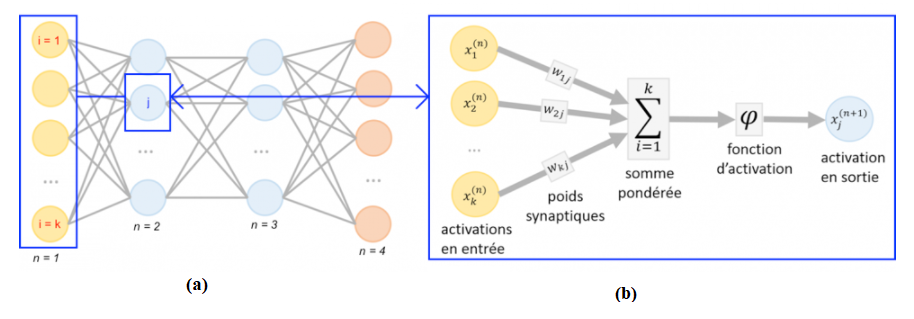
\includegraphics[width=0.9\linewidth]{./image_chapitre1/figure_02}
	\caption[(a) un NN organis� en 4 couches, (b) le m�canisme d'activation d'un neurone \cite{web01}]{(a) un NN organis� en 4 couches, (b) le m�canisme d'activation d'un neurone \cite{web01} }
	\label{fig:figure_02}
\end{figure}
\subsection{Le perceptron multi-couches}
Comme son nom l'indique le perceptron multi-couches (ou Multilayer Perceptron, souvent abr�g� � MLP �, en anglais) est un r�seau form� de plusieurs couches interm�diaires. Il consiste en un empilement de plusieurs neurones artificiels formant une couche cach�e. Chaque caract�ristique d'entr�e est connect�e � chaque neurone artificiel de la couche suivante. De m�me, les neurones artificiels de la couche cach�e sont tous connect�s aux neurones de couche de sortie \cite{web02}.
\begin{figure}[H]
	\centering
	\includegraphics[width=0.9\linewidth]{./image_chapitre1/figure_03}
	\caption[Un exemple de perceptron-multicouches constitu� de k couches \cite{web03}]{Un exemple de perceptron-multicouches constitu� de k couches \cite{web03}}
	\label{fig:figure_03}
\end{figure}
\section{Deep Learning}
\subsection{D�finition}
 Deep Learning ou apprentissage profond, est une branche du Machine Learning particuli�rement adapt�e � l'apprentissage de donn�es complexes en vue de r�aliser des mod�les avanc�s supervis�s ou non supervis�s  \cite{ref11}.\\[0.5\baselineskip]
Le perceptron multi-couches est l'exemple par excellence d'un mod�le d'apprentissage profond. Habituellement, un r�seau de neurones est consid�r� comme profond, s'il est compos� d'au moins quatre couches (c'est-�-dire trois couches cach�es + une couche de sortie) \cite{web02}.\\[0.5\baselineskip]
Celles-ci permettent de d�composer de mani�re hi�rarchique le contenu d'une donn�e complexe comme de la voix ou une image pour la classifier ensuite : identifier des mots pour la voix ou associer des tags descriptifs � des images.  Le Deep Learning sert le plus souvent � reconna�tre le langage, l'�criture et les images mais il peut aussi avoir d'autres usages dans les outils d'aide � la d�cision  \cite{ref12}.\\[0.5\baselineskip]
\subsection{R�tropropagation}
La r�tropropagation du gradient de l'erreur (ou backpropagation) est un algorithme d'optimisation permettant d'ajuster les param�tres d'un r�seau de neurones multicouches pour mettre en correspondance des entr�es et des sorties r�f�renc�es dans une base d'apprentissage.\\[0.5\baselineskip]
Pour pouvoir entra�ner ces syst�mes, il faut savoir comment ajuster les param�tres de chaque couche de neurones. Pour chaque exemple de donn�es (groupe d'observations de l'ensemble d'apprentissage), l'entr�e est donn�e au mod�le afin d'obtenir la sortie, celle-ci est compar�e avec le r�sultat attendu pour calculer l'erreur, La r�tropropagation permet de calculer le gradient de l'erreur pour chaque neurone, de la derni�re couche vers la premi�re (r�tropropagation). Cela permet de corriger les erreurs selon l'importance des �l�ments qui ont justement particip� � la r�alisation de ces erreurs. Ainsi, les poids qui contribuent � engendrer une erreur importante se verront modifi�s de mani�re plus significative que les poids qui ont engendr� une erreur marginale \cite{web04}.\\[0.5\baselineskip]
La d�riv�e par rapport � chaque coefficient $w$ est calcul�e en utilisant la r�gle de la cha�ne ou chain rule (voir figure \ref{fig:figure_04}.). Chaque coefficient est mis � jour comme suit:
\begin{eqnarray}
	w  \leftarrow  w - a \frac{\partial L(x,y)}{\partial w}
\end{eqnarray}
avec $L$ l'erreur, $w$ le coefficient, $x$ l'entr�e, $y$ la sortie et $a$ le taux d'apprentissage.
\begin{figure}[H]
	\centering
	\includegraphics[width=0.6\linewidth]{./image_chapitre1/figure_04}
	\caption[R�gle de la cha�ne]{R�gle de la cha�ne}
	\label{fig:figure_04}
\end{figure}
\textbf{Actualisation des coefficients:} Dans un r�seau de neurones, les coefficients sont actualis�s comme suit:
\begin{itemize}
	\item �tape 1 : Prendre un groupe d'observations appartenant aux donn�es d'entrainement
	\item �tape 2 : R�aliser la propagation avant pour obtenir le loss (valeur de la fonction de perte)  correspondant.
	\item �tape 3 : Effectuer une r�tropropagation du loss pour obtenir les gradients.
	\item �tape 4 : Utiliser les gradients pour actualiser les coefficients du r�seau
\end{itemize}
\subsection{Sur-apprentissage}
Un r�seau de neurones apprend gr�ce � des exemples (jeux d'entra�nements) qui lui sont soumis. Le but de cet apprentissage est de permettre au r�seau de tirer de ces exemples des g�n�ralisations et de pouvoir les appliquer � de nouvelles donn�es par la suite.\\[0.5\baselineskip]
On parle de sur-apprentissage (le terme anglais est overfitting) quand un mod�le a trop appris les particularit�s de chacun des exemples fournis en exemple. Il pr�sente alors un taux de succ�s tr�s important sur les donn�es d'entra�nement (pouvant atteindre jusqu'� 100\textdiscount, au d�triment de ses performances g�n�rales r�elles, et sur de nouvelles donn�es qu'il n'a pas encore vu, sa pr�diction sera totalement biais�e \cite{web05}. 
\subsection{Les diff�rentes architectures du Deep Learning}
Bien qu'il existe un grand nombre de variantes d'architectures pour l'apprentissage profond, il n'est pas toujours possible de comparer les performances de toutes les architectures, car elles ne sont pas toutes �valu�es sur les m�mes ensembles de donn�es. Le Deep Learning est un domaine � croissance rapide, et de nouvelles architectures, variantes ou algorithmes apparaissent toutes les semaines.
\section{Les r�seaux de neurones convolutifs}
      Les r�seaux de neurones convolutifs sont un type particulier de r�seau de neurones. D�sign�s par l'acronyme CNN, de l'anglais Convolutional Neural Network. Le nom de ces r�seaux vient du fait que leur fonctionnement est bas� sur l'utilisation d'une op�ration math�matique lin�aire appel�e convolution \cite{ref13}. \\[0.5\baselineskip]
Chaque couche - dite de convolution - balaye l'ensemble de la couche pr�c�dente en appliquant � chaque petite r�gion un m�me traitement local. Dans le cas d'un texte, les r�gions sont les n-grammes de la phrase. Pour une image, ils comportent deux parties bien distinctes, en entr�e, une image est fournie sous la forme d'une matrice de pixels. Elle a 2 dimensions pour une image en niveaux de gris. La couleur est repr�sent�e par une troisi�me dimension, de profondeur 3 pour repr�senter les couleurs fondamentales [Rouge, Vert, Bleu].
\begin{figure}[H]
	\centering
	\includegraphics[width=0.9\linewidth]{./image_chapitre1/figure_05}
	\caption[Architecture standard d'un r�seau de neurone convolutif \cite{web06}]{Architecture standard d'un r�seau de neurone convolutif \cite{web06}}
	\label{fig:figure_05}
\end{figure}
\subsection{L'op�ration de convolution}
Les r�seaux de neurones classiques ne s'adaptent pas parfaitement aux images compl�tes. Par exemple, certaines bases de donn�es (comme CIFAR-10) ont des images de taille 32 x 32 x 3 (32 pixels de largeur, 32 de hauteur, 3 canaux de couleurs), de sorte qu'un seul neurone enti�rement connect� dans une premi�re couche cach�e d'un r�seau de neurones ordinaire aurait 32 * 32 * 3 = 3072 poids. Si cette quantit� semble toujours g�rable dans ce cas de figure, il est clair que cette structure enti�rement connect�e ne s'adapte pas aux images plus grandes. En effet, avec une image de taille plus commune, par exemple 200 x 200 x 3, ceci conduirait � avoir des neurones avec 200 * 200 * 3 = 120 000 poids. Avec plus de neurones, ces param�tres s'additionneraient tr�s rapidement. Cette connectivit� totale prend beaucoup de temps et le nombre consid�rable de param�tres conduirait sans doute � un surapprentissage \cite{ref14}.
\subsection{Architecture CNN}
Une architecture CNN est form�e par un empilement de couches de traitement ind�pendantes:
\begin{itemize}
	\item La couche de convolution (CONV) est la  la composante cl� d'un r�seau de neurones convolutif. Elle effectue la majeure partie des lourdes t�ches de calcul. La couche de convolution re�oit en entr�e plusieurs images, et calcule la convolution de chacune d'entre elles avec chaque filtre. Les filtres correspondent aux caract�ristiques (features) que l'on souhaite retrouver dans les images. La sortie r�sultante est appel�e carte de caract�ristiques (en anglais activation map ou feature map), et nous indique o� se situent ces features. Une couche convolutive est constitu�e de plusieurs filtres (ou noyaux) de convolution � appliquer sur une matrice d'entr�e (une image ou une feature map pr�c�dente). Les noyaux des filtres d�signent les poids de la couche de convolution. Ils sont initialis�s puis mis � jour par \textbf{la descente du gradient} \cite{ref15}.\\
	La convolution peut �tre ajust�e selon certains param�tres, dont le nombre et la taille de filtres, le stride et le padding .Le stride est un param�tre indiquant de combien de pas on se d�place entre deux calculs de la convolution, et le padding indique combien de rang�es de 0 on ajoute autour de l'entr�e (Cette marge permet de contr�ler la dimension spatiale du volume de sortie).
	\begin{figure}[H]
		\centering
		\includegraphics[width=0.9\linewidth]{./image_chapitre1/figure_06}
		\caption[Op�ration de convolution En rouge : image en input. En bleu : le filtre de convolution. En violet : r�sultat de l'application du filtre sur la partie de l'image s�lectionn�e \cite{web07}]{Op�ration de convolution En rouge : image en input. En bleu : le filtre de convolution. En violet : r�sultat de l'application du filtre sur la partie de l'image s�lectionn�e \cite{web07}}
		\label{fig:figure_06}
	\end{figure}

\item La couche d'activation : Il est possible d'am�liorer l'efficacit� du traitement en intercalant entre les couches de traitement une couche qui va op�rer une fonction math�matique (fonction d'activation) sur les signaux de sortie.\\
La fonction d'activation d'unit� lin�aire rectifi�e ou couche ReLU pour Rectified Linear Unit Layer est certainement la plus utilis�e dans les CNN. C'est une couche dite de correction qui force les neurones � retourner des valeurs positives \cite{ref16}.


\begin{figure}[H]
	\centering
	\includegraphics[width=0.9\linewidth]{./image_chapitre1/figure_07}
	\caption[Types de fonctions d'activation \cite{web07}]{Types de fonctions d'activation \cite{web07}}
	\label{fig:figure_07}
\end{figure}

\item La couche de pooling (POOL), qui permet de compresser l'information en r�duisant la taille de l'entr�e interm�diaire (souvent par sous-�chantillonnage), r�duisant ainsi la quantit� de param�tres et de calcul dans le r�seau. Il est fr�quent de trouver dans les architectures de CNN des couches POOL ins�r�es p�riodiquement entre deux couches convolutives successives. 
Il existe plusieurs types de pooling, les plus populaires sont le max-pooling et l'average-pooling.
\begin{figure}[H]
	\centering
	\includegraphics[width=0.8\linewidth]{./image_chapitre1/figure_08}
	\caption[Pooling avec un filtre 2x2 et un pas de 2]{Pooling avec un filtre 2x2 et un pas de 2 \cite{ref17}}
	\label{fig:figure_08}
\end{figure}
\item 	La couche "enti�rement connect�e" (en anglais fully connected layer) (FC) s'applique sur une entr�e pr�alablement aplatie o� chaque entr�e est connect�e � tous les neurones. Les couches de fully connected sont typiquement pr�sentes � la fin des architectures de CNN et peuvent �tre utilis�es pour optimiser des objectifs tels que les scores de classe.
\newpage
\begin{figure}[H]
	\centering
	\includegraphics[width=0.7\linewidth]{./image_chapitre1/figure_09}
	\caption[Exemple de couche fully connected CNN \cite{web07}]{Exemple de couche fully connected CNN \cite{web07}}
	\label{fig:figure_09}
\end{figure}
\textbf{La mise � plat (Flattening)}\\[0.5\baselineskip]
Il consiste simplement � mettre � bout toutes les entr�es que nous avons pour en faire un (long) vecteur. 
\begin{figure}[H]
	\centering
	\includegraphics[width=0.7\linewidth]{./image_chapitre1/figure_10}
	\caption[Mise � plat des images \cite{web08}]{Mise � plat des images \cite{web08}}
	\label{fig:figure_10}
\end{figure}
\item La couche de perte (LOSS) sp�cifie comment l'entrainement du r�seau p�nalise l'�cart entre le signal pr�vu et r�el. Elle est normalement la derni�re couche dans le r�seau. Diverses fonctions de perte adapt�es � diff�rentes t�ches peuvent y �tre utilis�es. La fonction � Softmax � g�n�ralement utilis�e pour l'optimisation de r�seau de classification d'images, elle permet de calculer la distribution de probabilit�s sur les classes de sortie.
\end{itemize}

\section{L'analyse des donn�es du big data}
A la lumi�re du volume important de donn�es du big data il est n�cessaire d'utiliser des moyens d'analyse diff�rents des m�thodes d'analyse traditionnelles.\\[0.5\baselineskip]
Tout d'abord l'utilisation de l'Intelligence Artificielle ou IA qui peut se d�finir comme une discipline scientifique relative au traitement des connaissances et au raisonnement, dans le but de permettre � une machine d'ex�cuter des fonctions normalement associ�es � l'intelligence humaine : compr�hension, raisonnement, dialogue, adaptation, apprentissage, etc. Les programmes d'IA apprennent � partir des donn�es afin de r�pondre intelligemment aux nouvelles donn�es et ainsi fournir des r�sultats correspondants.\\[0.5\baselineskip]
Un des moyens d'application de l'IA est l'apprentissage automatique et l'apprentissage profond. Gr�ce � l'apprentissage automatique, les ordinateurs apprennent sans �tre explicitement programm�s. Lorsque nous achetons en ligne, l'apprentissage automatique permet de recommander d'autres produits qui pourraient nous int�resser en fonction des produits que nous avons d�j� achet�s. Lorsque nous utilisons notre carte de cr�dit, l'apprentissage automatique compare la transaction � une base de donn�es de transactions telles que la zone g�ographique habituelle de transactions et ainsi permet la d�tection des fraudes. Lorsque notre voiture nous indique la dur�e d'un trajet jusqu'� notre domicile, l'apprentissage automatique permet de d�terminer o� se trouve notre domicile. L'apprentissage automatique est un sous domaine de l'intelligence artificielle. Le Deep Learning est lui-m�me une sous-cat�gorie de l'apprentissage automatique. L'exemple d'application le plus commun est la reconnaissance visuelle. Par exemple, un algorithme va �tre programm� pour d�tecter certains visages depuis les images en provenance d'une cam�ra. Suivant la base de donn�es attribu�e, il pourra rep�rer un individu recherch� dans une foule, d�tecter le taux de satisfaction � la sortie d'un magasin en d�tectant les sourires, etc. Un ensemble d'algorithmes pourra �galement reconna�tre la voix, le ton, l'expression d'un questionnement, d'une affirmation ainsi que les mots d'une conversation.\\[0.5\baselineskip]
Pour r�sumer, le volume de donn�es composant le big data peut �tre consid�r� comme difficilement exploitable sans un support informatique. L'IA est donc l'intelligence qui permet une exploitation efficace du big data, et l'apprentissage automatique et  profond font partie des techniques qui facilitent l'analyse du big data \cite{web09}.
\section{Limites du machine learning dans le Big Data}
Les algorithmes de machine Learning ne sont pas non plus une boite noire magique qui permet de tout deviner et qui s'adapte � tout. Si l'on souhaite faire des pr�dictions de bonne qualit�, il y a certaines choses � prendre en compte.\\[0.5\baselineskip]
Tout d'abord, il est n�cessaire que les r�sultats que l'on souhaite pr�dire soient diff�rentiables. Les algorithmes ne jouent que 20\% dans la qualit� des pr�dictions, les 80\% autres sont dus � la qualit� des donn�es. \\[0.5\baselineskip]
Dans le monde r�el, les choses sont bien plus complexes, on peut avoir des impr�cisions sur les caract�ristiques, des erreurs dans la classification des donn�es ou beaucoup d'autres facteurs qui rendent les pr�dictions moins �videntes. Une autre limite du Machine Learning est que les algorithmes sont incapables d'extrapoler les grands volumes de donn�es de mani�re fiable. Il est donc n�cessaire de faire des pr�dictions uniquement sur le m�me domaine de donn�es que celui utilis� pour l'apprentissage. Les algorithmes de machine Learning ne permettent donc pas d'apprendre de nouvelles choses mais seulement d'automatiser des choses connues ou de mettre en �vidence des relations. Dans ce contexte, il est essentiel que les m�thodes d'apprentissage puissent suivre le rythme des donn�es, non seulement en termes de volume, mais aussi de la vitesse � laquelle elles sont g�n�r�es et trait�es, afin d'�tre utiles.\\[0.5\baselineskip]
Les m�thodes classiques de machine learning ont �t� r�cemment adapt�es aux propri�t�s du Big Data en appliquant la philosophie Deep learning. Cette derni�re vise � produire des repr�sentations abstraites des caract�ristiques observ�es, qui sont organis�s en couches; plus la couche est �lev�e, plus le niveau d'abstraction est �lev�. Bien que le Deep Learning ait �t� appliqu� dans une panoplie de domaines et ait donn� des r�sultats appr�ciables, il a certains inconv�nients. En fait,  les couches superpos�es cach�es sont consid�r�es comme une bo�te noire dont la taille et les param�tres sont d�finis empiriquement. De plus, la signification de chaque variable latente (cach�e/non observ�e), dans une couche cach�e, est perdue et l'interpr�tabilit� de la repr�sentation des caract�ristiques abstraites est pratiquement impossible \cite{ref18}.\\[0.5\baselineskip]
Construire des mod�les d'apprentissage automatique � partir de grandes masses de donn�es (Big Data) n�cessite le d�veloppement de nouveaux types d'algorithmes. La plupart des algorithmes d'apprentissage automatique ne passent pas � l'�chelle \cite{ref12}, elles ne sont pas suffisamment performantes pour exploiter pleinement la valeur du Big Data, sa variabilit� et sa v�racit� rendent le processus de machine learning perplexe. Le volume de donn�es est trop large pour des analyses compl�tes, et les corr�lations et relations entre ces donn�es sont trop importantes pour que les analystes puissent tester toutes les hypoth�ses afin de d�gager une valeur de ces donn�es. Les outils d'apprentissage profond ont acquis une attention consid�rable dans l'apprentissage machine appliqu�. Toutefois, ces outils ne tiennent pas compte de l'incertitude du mod�le, c'est l� o� les r�seaux bay�siens semblent id�aux pour exploiter les opportunit�s cach�es du Big Data.
\section{Les r�seaux bay�siens}
\subsection{C'est quoi un r�seau bay�sien ?}
On peut d�finir un r�seau bay�sien par un mod�le graphique regroupant au sein d'un m�me formalisme la th�orie des graphes et celle des probabilit�s afin de fournir des outils efficaces autant qu'intuitifs pour repr�senter une distribution de probabilit�s jointe sur un ensemble de variables al�atoires. Ce formalisme tr�s puissant permet une repr�sentation intuitive de la connaissance sur un domaine d'application donn� et facilite la mise en place de mod�les performants et clairs. La repr�sentation de la connaissance se base sur la description, par des graphes, des relations de causalit� existant entre des variables d�crivant le domaine d'�tude. A chaque variable est associ�e une distribution de probabilit�s locale quantifiant la relation causale \cite{ref19}.
\subsection{Pourquoi les r�seaux bay�siens ?}
Une des grandes probl�matiques de notre �poque est de traiter la grande quantit� des donn�es qui est mise � notre disposition (notamment gr�ce � l'informatique) pour en extraire de l'information. Il serait donc int�ressant d'avoir un (ou plusieurs) mod�le(s) effectuant le lien entre les observations et la r�alit� pour un objectif pr�cis, et cela, m�me lorsque les observations sont incompl�tes et/ou impr�cises.\\[0.5\baselineskip]
Imaginons un statisticien qui veut analyser un tableau de mesures pour une population donn�e. Il se retrouve face � une immense masse d'informations de laquelle il doit extraire de la connaissance ! Il va donc essayer de retrouver les relations pertinentes entre des variables ou des groupes de variables. L'utilisation des r�seaux bay�siens va lui permettre d'obtenir une repr�sentation compacte de ces ensembles de d�pendances gr�ce � la notion de probabilit�s conditionnelles, � partir de laquelle il lui sera plus simple de raisonner.\\[0.5\baselineskip]
Les r�seaux bay�siens permettent donc de transformer en mod�le interpr�table la connaissance contenue dans des donn�es.\\[0.5\baselineskip]
Les r�seaux probabilistes sont �galement une repr�sentation du savoir incertain plus flexible que les syst�mes � base de r�gles. Par exemple, en m�decine, une m�me combinaison de sympt�mes peut �tre observ�e pour diff�rentes maladies.\\[0.5\baselineskip]
Prenons l'exemple du corps humain, syst�me complexe � volont�. Lorsqu'un individu est malade, nous allons observer pour celui-ci un certain nombre de grandeurs (tension, fi�vre, etc). En fonction de ces diff�rentes observations et de sa connaissance a priori le m�decin va donner son diagnostic. Ce diagnostic est ici �valu� en fonction d'un nombre restreint de param�tres, or il se peut que deux individus aient la m�me forme (les m�mes valeurs pour toutes les grandeurs observ�es) et que l'un d'eux soit malade, tandis que l'autre est sain.\\[0.5\baselineskip]
Les mod�les probabilistes ont cet avantage de fournir syst�matiquement une probabilit� � chaque �tat (ici sain ou malade). Celle-ci peut alors �tre consid�r�e comme un indice de confiance dans le r�sultat (par exemple, cet individu a 85\% de chance d'�tre malade). Bien s�r un tel diagnostic n'est pas satisfaisant d'un point de vue �thique pour d�cider d'administrer ou non un traitement.\\[0.5\baselineskip]
Pour r�sumer:
\begin{itemize}
	\item L'aspect graphique des mod�les bay�siens permet de repr�senter les relations      entre les attributs clairement et intuitivement.
	\item Leurs orientations (si elles existent) peuvent repr�senter des relations de cause � effet.
	\item Les mod�les probabilistes sont capables de g�rer l'incertain et l'impr�cis \cite{ref20}.
\end{itemize}
\section{Formalisme math�matique}
\subsection{D�finition formelle (R�seaux bay�siens)}
Un r�seau bay�sien $ B = (G, \theta) $ est d�fini par:
\begin{itemize}
	\item une structure $ G = (V, E) $ qui est un graphe orient� sans circuit (DAG : Directed Acyclic Graph) o� $V$ est l'ensemble des n\oe{}uds qui repr�sentent un ensemble de variables al�atoires $ X = (X_1, ..., X_n) $  et $E$ est l'ensemble des arcs,
	\item et des param�tres $ \theta = [ P (X_i /Pa(X_i))  ] $ qui sont des distributions de probabilit�s pour que B v�rifie la condition de Markov.
\end{itemize}
De mani�re plus g�n�rale, les r�seaux bay�siens (RB) sont des mod�les graphiques pour repr�senter les relations probabilistes parmi un ensemble de variables al�atoires. Les RB offrent une repr�sentation graphique de mani�re compacte des lois de probabilit� jointes entre variables. La distribution de probabilit�s sur l'ensemble des variables est d�finie par:
\begin{eqnarray}
 P(X_1,X_2, ...,X_n) = \prod_{i=1}^n P(X_i/Pa(X_i))
\end{eqnarray}
O� $Pa(X_i)$est l'ensemble des parents du n\oe ud $Xi$ dans $G$ \cite{ref21}.
\begin{figure}[H]
	\centering
	\includegraphics[width=0.6\linewidth]{./image_chapitre1/figure_13}
	\caption[Exemple de r�seau bay�sien]{Exemple de r�seau bay�sien}
	\label{fig:figure_11}
\end{figure}
\section{Conclusion}
Dans ce chapitre, nous avons d�fini le concept d'analyse des big data. Par la suite, nous avons proc�d� � de brefs rappels sur les approches du data mining, leurs d�finitions, m�thodes, applications dans le big data et leurs limites ainsi que des rappels sur les r�seaux bay�siens.




























\include{pagevide}
\chapter{\sc Les r�seaux bay�siens profonds }\label{chap2} 
\section{Introduction}
Nous introduisons dans ce second chapitre la notion des r�seaux bay�siens profonds, nous citons quelques travaux associ�s, nous effectuons par la suite une description de l'�tat de l'art des approches utilis�es pour l'impl�mentation des r�seaux bay�siens profonds et plus particuli�rement l'approche de Monte Carlo Dropout.
\section{Les r�seaux bay�siens profonds }
La principale motivation derri�re la prise en compte des r�seaux bay�siens profonds (Deep Bayesian Networks en anglais) est la n�cessit� de fournir une mod�lisation simplifi�e et pr�cise des donn�es de grande dimension. Les d�fis des Big Data n�cessitent un mod�le robuste qui est appris � partir des donn�es volumineuses captur�es dans un petit intervalle de temps. \\[0.5\baselineskip]
Il existe deux approches majeures pour l'apprentissage des r�seaux bay�siens profonds. La premi�re approche c'est d'apprendre une structure du r�seau bay�sien profond en proposant ses propres algorithmes de clustering \cite{ref18}. La deuxi�me approche est d'ajouter l'aspect bay�sien aux architectures existantes du deep learning que nous appelons \textbf{l'apprentissage profond bay�sien} \cite{ref34}.
\section{Travaux associ�s}
\subsection{Architecture du r�seau bay�sien profond pour le Big data mining \cite{ref18}}
Dans cet article les auteurs se sont inspir�s du principe de l'apprentissage et des r�seaux bay�siens hi�rarchiques afin de fournir une nouvelle architecture de r�seau bay�sien multi-couches avec des variables latentes. Cette architecture est appel�e  Deep Bayesian Network (Deep-BN). Il s'agit en effet d'un r�seau bay�sien arborescent o� toutes les variables sont r�parties en un nombre fini de couches; la couche la plus basique est compos�e de toutes les caract�ristiques observ�es. Ils ont propos� �galement une m�thode triviale et nouvelle pour l'apprentissage de cette architecture. Ils pr�sentent une �tape de regroupement de caract�ristiques qui vise � trouver les groupes de variables tr�s d�pendantes et une �tape d'apprentissage de variables latentes qui trouve la distribution de probabilit� des nouvelles variables cach�es abstraites. Le nombre d'it�rations de ces �tapes, c'est-�-dire le nombre de couches cach�es, d�pend de la quantit� de perte d'information entre deux couches successives. Par cons�quent, leur architecture a l'avantage d'�tre simplement apprise et facilement interpr�t�e en raison de l'aspect graphique du r�seau bay�sien. Celui ci permet de r�duire la dimension des fonctions dans un contexte de m�ga donn�es tout en conservant le plus d'information possible. Il offre �galement un rendement am�lior� en mati�re de classification.
\subsection{R�seau de neurones bay�sien � convolution profonde pour l'analyse de la qualit� des SMS \cite{ref27}}
Pour obtenir une communication pratique et �conomique, le short message service (SMS) est l'un des moyens les plus faciles et les plus r�alisables. Cependant, de plus en plus de messages ind�sirables tels que la publicit� constituent un  plus grand d�fi pour ce service. Dans cet article, les auteurs ont propos� une nouvelle architecture de r�seau de neurones convolutifs "Convolutional neural network (CNN)" bas�e sur l'apprentissage bay�sien pour r�aliser une �valuation de la qualit� des SMS. Plus pr�cis�ment, ils forment d'abord le vecteur de mot de chaque mot dans l'ensemble de donn�es du SMS, et convertissent le groupe de vecteurs de mots de chaque SMS en une matrice bidimensionnelle. Par la suite, la matrice de caract�ristiques est utilis�e comme entr�e dans le r�seau de neurones convolutifs, dans lequel les caract�ristiques du SMS sont extraites par les noyaux de convolution, et l'extraction des caract�ristiques est simplifi�e par l'algorithme bay�sien. Enfin, le score de qualit� peut �tre atteint en fonction des caract�ristiques optimales locales.
\newpage
\subsection{Construction des r�seaux de neurones profonds par l'apprentissage de la structure d'un r�seau bay�sien \cite{ref33}}
Il existe deux approches qui ont �t� �tudi�es pour l'apprentissage de la structure des mod�les graphiques probabilistes. Plus pr�cis�ment, les r�seaux bay�siens pour l'estimation de la densit� et la d�couverte des causes: L'une bas�e sur les scores et l'autre sur les contraintes. Motiv�s par les deux m�thodes d'apprentissage de la structure des mod�les graphiques probabilistes. Ces auteurs ont propos� une interpr�tation de la profondeur et de la connectivit� inter-couches dans les r�seaux de neurones profonds pour en extraire un Algorithme d'apprentissage de la structure de telle sorte qu'une hi�rarchie des ind�pendances dans la distribution d'entr�es est encod�e dans un graphe g�n�ratif profond, o� les ind�pendances d'ordre inf�rieur sont encod�es dans des couches plus profondes. Ainsi, le nombre de couches est automatiquement d�termin�, ce qui est souhaitable dans toute m�thode d'apprentissage de l'architecture.\\[0.5\baselineskip]
Les auteurs commencent par convertir le graphe g�n�ratif en un graphe discriminant, d�montrant la capacit� de ce dernier � imiter (pr�server les d�pendances conditionnelles) du premier. Dans la structure r�sultante, un neurone dans une couche est autoris� � se connecter aux neurones dans des couches plus profondes en sautant des couches interm�diaires. En outre, les neurones des couches plus profondes repr�sentent des ind�pendances d'ordre faible (petits ensembles de conditions) et ont une large port�e d'entr�e, tandis que les neurones des premi�res couches repr�sentent des ind�pendances d'ordre sup�rieur (ensembles de conditions plus grands) et ont une port�e plus �troite.
\subsection{Reconnaissance faciale avec les r�seaux convolutifs bay�siens pour des syst�mes de surveillance robustes \cite{ref34}}
La reconnaissance abstraite des images faciales est l'un des probl�mes de recherche les plus difficiles dans les syst�mes de surveillance en raison de diff�rents probl�mes, notamment la pose, l'expression, l'�clairage et la r�solution. Le processus de reconnaissance faciale consiste � identifier la personne en comparant certaines caract�ristiques d'une nouvelle personne (�chantillon d'entr�e) avec les personnes connues dans la base de donn�es. La robustesse de la m�thode de reconnaissance repose fortement sur la force des caract�ristiques extraites et la capacit� de traiter des images de visage de faible qualit�. La capacit� d'apprendre des caract�ristiques robustes � partir d'images brutes du visage rend les r�seaux neuronaux convolutionnels profonds (Dcnns) attrayants pour la reconnaissance du visage.\\[0.5\baselineskip]
\cite{ref34} ont utilis� la m�thode dropout (le d�crochage) pour former une architecture DCNN bay�sien (B-DCNN). Il est montr� qu'il y'a une relation entre le dropout et l'inf�rence variationnelle dans les B-DCNNs avec les distributions de Bernoulli sur les poids du r�seau. Dans ce travail, les auteurs ont utilis� cette approche pour repr�senter les incertitudes du mod�le tout en classant les images faciales. Le d�crochage est �galement utilis� au moment du test pour �chantillonner la distribution post�rieure sur les poids. La moyenne et la variance des �chantillons sont utilis�es respectivement comme confiance et incertitude pour chaque classe. La d�cision finale de classification est prise sur la base d'une fonction heuristique simple.
\subsection{R�seaux de neurones bay�siens convolutifs avec inf�rence variationnelle approximative de Bernoulli \cite{ref35}}
Les r�seaux de neurones convolutifs (CNNs) fonctionnent bien sur de grands ensembles de donn�es. Mais les donn�es �tiquet�es sont difficiles � collecter. Donc le probl�me qui se pose est alors de savoir comment utiliser les CNNs avec de petits ensembles de donn�es - car les CNNs tombent dans le surapprentissage rapidement. Dans cet article, les auteurs pr�sentent un CNN bay�sien efficace, offrant une r�sistance face au surapprentissage sur des petits ensembles de donn�es contrairement aux anciennes approches. Pour ce faire, ils commencent par placer une distribution de probabilit� sur les noyaux du CNN. Ils pr�sentent de nouveaux r�sultats th�oriques utilisant le dropout lors de l'apprentissage des r�seaux autant qu'une inf�rence approximative dans les r�seaux de neurones bay�siens. Cela a permet de r�aliser le mod�le employ� dans cet \oe{}uvre en utilisant les outils existants sur le terrain sans augmentation de la complexit� temporelle. Ils approximent la partie post�rieure intraitable du mod�le avec les distributions variationnelle de Bernoulli, sans avoir besoin de param�tres suppl�mentaires. Les r�sultats montrent une am�lioration consid�rable de la pr�cision de la classification par rapport aux techniques standards utilis�es sur le CIFAR10.
\subsection{Bayesian SegNet : Incertitude du mod�le dans les architectures d'encodeurs-d�codeurs convolutifs profonds pour la compr�hension des sc�nes \cite{ref36}}
Dans cet article, ils pr�sentent un cadre d'apprentissage profond pour la segmentation s�mantique probabiliste en pixels, qu'ils appellent Bayesian SegNet. La segmentation s�mantique est un outil important pour la compr�hension de la sc�ne visuelle et une mesure significative de l'incertitude est essentielle pour la prise de d�cision. Cette contribution est un syst�me pratique qui est capable de pr�dire les �tiquettes de classe pixel par pixel avec une mesure de l'incertitude du mod�le en utilisant l'apprentissage bay�sien profond. Ils parviennent par un �chantillonnage Monte Carlo avec le dropout au moment du test pour g�n�rer une distribution post�rieure des �tiquettes des classes de pixels. Ils montrent aussi que l'incertitude de la mod�lisation am�liore les performances de segmentation de 2 � 3 \% pour un certain nombre d'ensembles de donn�es et d'architectures tels que SegNet, FCN, Dilation Network et DenseNet.
\subsection{Le dropout comme approximation bay�sienne : Repr�sentation de l'incertitude du mod�le dans l'apprentissage profond \cite{ref37}}
Les outils d'apprentissage profond ont acquis une attention consid�rable dans les applications de l'apprentissage machine. Toutefois, ces outils de r�gression et de classification ne tiennent pas compte de l'incertitude du mod�le. En comparaison, les mod�les bay�siens offrent un cadre math�matiquement pour estimer l'incertitude du mod�le, mais viennent g�n�ralement avec un co�t de calcul �norme. Dans cet article, les auteurs d�veloppent un nouveau cadre th�orique qui permet d'utiliser le dropout dans les r�seaux de neurones profonds (NNs) comme inf�rence bay�sienne approximative dans les processus gaussiens profonds. Un r�sultat direct de cette th�orie, donne des outils pour mod�liser l'incertitude avec les r�seaux de neurones profonds en extrayant des informations des mod�les existants qui ont �t� n�glig�s jusqu'� pr�sent. Cela permet de r�duire le probl�me de la repr�sentation de l'incertitude dans l'apprentissage profond sans sacrifier ni la complexit� du calcul ni la pr�cision des tests. Ils r�alisent dans cet ?uvre, une �tude approfondie des propri�t�s de l'incertitude du Dropout. Diverses architectures de r�seau sont �valu�es sur des t�ches de r�gression et de classification, en utilisant le MNIST comme exemple. Ils approuvent une am�lioration consid�rable de la fonction pr�dictive du log-vraisemblance ainsi que sur l'erreur quadratique moyenne par rapport aux m�thodes existantes.
\subsection{G�n�ration de conversation �motionnelle bas�e sur un r�seau neuronal bay�sien profond \cite{ref38}}
Le domaine de la g�n�ration de conversations � l'aide de r�seaux neuronaux attire de plus en plus l'attention des chercheurs depuis plusieurs ann�es. Cependant, les mod�les de langage neuronal traditionnels ont tendance � g�n�rer une r�ponse g�n�rique avec une mauvaise logique s�mantique et aucune �motion. Cet article propose un mod�le de g�n�ration de conversation �motionnelle bas� sur un r�seau neuronal bay�sien profond qui peut g�n�rer des r�ponses avec des �motions riches, des th�mes clairs et des phrases diverses. Le sujet et les mots-cl�s �motionnels des r�ponses sont pr�-g�n�r�s en introduisant la connaissance du bon sens dans le mod�le. La r�ponse est divis�e en plusieurs clauses, puis un g�n�rateur multidimensionnel bas� sur le m�canisme transformateur propos� dans cet article est utilis� pour g�n�rer it�rativement des clauses � partir de deux dimensions : la granularit� des phrases et la structure des phrases. Les exp�riences subjectives et objectives prouvent que, par rapport aux mod�les existants, le mod�le propos� am�liore efficacement la logique s�mantique et la pr�cision �motionnelle des r�ponses. Ce mod�le am�liore �galement consid�rablement la diversit� des r�ponses, en surmontant largement les lacunes des mod�les traditionnels qui g�n�rent des r�ponses s�res.
\section{L'apprentissage profond bay�sien}
Le DEEP Learning a obtenu un succ�s significatif dans de nombreuses t�ches de perception, y compris la reconnaissance visuelle des objets, la compr�hension de  textes et la reconnaissance vocale. Il s'agit sans aucun doute de t�ches fondamentales pour un syst�me complet d'intelligence artificielle (IA) ou d'ing�nierie des donn�es (DE) fonctionnel. Cependant, pour construire un v�ritable syst�me d'IA/DE, le simple fait de pouvoir voir, lire et entendre est loin d'�tre suffisant. Il devrait surtout avoir la capacit� de penser.\\[0.5\baselineskip]
Dans presque tous les probl�mes du monde r�el, ce que nous voulons, ce n'est pas seulement un r�sultat, mais nous avons aussi besoin d'une connaissance de la confiance / certitude dans ce r�sultat. Lorsque l'apprentissage profond est utilis� dans des domaines sensibles tels que la sant� et le contr�le autonome, nous devrions nous interroger non seulement sur la pr�cision mais aussi sur la confiance des mod�les d�ploy�s.\\[0.5\baselineskip]
Prenons l'exemple du diagnostic m�dical. En plus de voir des sympt�mes visibles (ou des images m�dicales) et d'entendre des descriptions de patients, un m�decin doit rechercher des relations entre tous les sympt�mes et de pr�f�rence inf�rer l'�tiologie correspondante. Seulement apr�s cela le m�decin peut fournir des conseils m�dicaux pour les patients. Dans cet exemple, bien que les capacit�s de voir et d'entendre permettent au m�decin d'acqu�rir de l'information aupr�s des patients, c'est la partie de la pens�e qui d�finit un m�decin. En particulier, la capacit� de penser ici pourrait impliquer l'inf�rence causale, la d�duction logique et le traitement de l'incertitude, ce qui est apparemment au-del� de la capacit� des m�thodes conventionnelles d'apprentissage en profondeur.\\[0.5\baselineskip]
Un autre exemple, nous aimerions qu'un v�hicule autonome non seulement identifie correctement les objets dans son environnement, mais fournisse �galement une mesure de l'incertitude. De m�me, si nous �crivons un bot qui n�gocie sur le march� de la bourse, nous voulons qu'il reconnaisse, quand la situation sort de sa zone de confort, de sorte qu'il peut arr�ter d'agir et ne pas faire faillite.\\[0.5\baselineskip]
Une grande partie de l'intelligence n'agit pas quand on est incertain. Il est donc surprenant que pour de nombreux projets de ML, exprimer l'incertitude n'est pas ce qui est vis�.\\[0.5\baselineskip]
Les outils standards d'apprentissage profond pour la r�gression et la classification ne saisissent pas l'incertitude du mod�le. Dans la classification, les probabilit�s pr�dictives obtenues � la fin (la sortie softmax) sont souvent interpr�t�es � tort comme une confiance du mod�le (si c'est 0,8, alors mon mod�le est s�r � 80 \% de sa pr�diction). Yarin Gal \cite{web10} argumente, qu'un mod�le peut �tre incertain dans ses pr�dictions m�me avec une sortie softmax �lev�e.\\[0.5\baselineskip]
Heureusement, un autre type de mod�les existe, les mod�les bay�siens, qui excellent dans l'inf�rence et la gestion de l'incertitude. Le probl�me est que le mod�le bay�sien n'est pas aussi bon que les mod�les d'apprentissage profond pour les t�ches de perception. Pour r�soudre le probl�me, il est donc naturel d'int�grer �troitement l'apprentissage profond et le mod�le bay�sien dans un cadre probabiliste fond� sur des principes, que nous appelons l'apprentissage profond bay�sien (BDL).\\[0.5\baselineskip]
L'id�e principale de l'apprentissage profond bay�sien est d'introduire la notion de probabilit� durant la phase d'entra�nement et la phase de pr�diction du r�seau. Pour ce faire, les instances manipul�es sont des distributions de probabilit�s et non des scalaires. Ainsi, les poids du r�seau et les valeurs contenues des neurones suivent des lois normales qui sont caract�ris�es par une valeur moyenne et un �cart-type.
Ceci constitue la seule diff�rence conceptuelle notable entre l'apprentissage profond et l'apprentissage profond bay�sien (les autres diff�rences �tant d'ordre math�matique et algorithmique). Finalement, chaque neurone de la couche de sortie du r�seau retourne une loi normale dont la valeur moyenne et l'�cart type ont une valeur d�termin�e par l'image d'entr�e du r�seau. De ces distributions, il est possible � l'aide de formules math�matiques de calculer les diff�rentes incertitudes \cite{web11}.\\[0.5\baselineskip]
Plusieurs formulations bay�siennes r�centes du deep learning fournissent des techniques alternatives pour extraire des estimations d'incertitude � partir des r�seaux profonds, y compris l'approche de Monte Carlo Dropout \cite{ref37} (qui sera d�velopp�e par la suite), pr�c�demment employ�e dans l'apprentissage actif profond pour la classification des images \cite{ref39} et la reconnaissance des entit�s d�sign�es \cite{ref40} et l'approche de Bayes-by-Backprop.\cite{ref41}.
\section{Monte Carlo Dropout comme approximation bay�sienne}
\subsection{Dropout}
C'est une technique de r�gularisation (pour combattre l'overfitting) dont le principe est de d�sactiver al�atoirement � chaque it�ration un certain pourcentage des neurones d'une couche. Cela �vite ainsi la sur-sp�cialisation d'un neurone (et donc l'apprentissage par c\oe ur) \cite{ref42}. Il faut que la probabilit� qu'un neurone ne soit pas d�sactiv� soit entre 0.5 et 0.8 pour obtenir les meilleurs r�sultats \cite{ref43}. Ceci peut se faire par un tirage al�atoire. Par exemple, en jetant une pi�ce pour d�cider de la d�sactivation d'un neurone, on obtiendrait une probabilit� de 0.5. Le nombre de neurones est donc r�duit mais de fa�on al�atoire � chaque it�ration d'apprentissage. Cette technique fonctionne bien dans la g�n�ralisation d'un r�seau.
\newpage
\begin{figure}[H]
	\centering
	\includegraphics[width=0.9\linewidth]{./image_chapitre1/figure_11}
	\caption[Un r�seau de neurones lors de l'application de la technique de Dropout]{Un r�seau de neurones lors de l'application de la technique de Dropout \cite{ref43}}
	\label{fig:figure_11}
\end{figure}
Cette technique n'est utilis�e que pendant la phase d'apprentissage. Le r�seau neuronal se voit amput� d'une partie de ses neurones pendant la phase d'entrainement (leur valeur est estim�e � 0) et ils sont par contre r�activ�s pendant la phase de test.
\subsection{Estimation d'incertitude}
La notion d'incertitude en apprentissage automatique se divise en deux cat�gories: les incertitudes �pist�miques et les incertitudes al�atoires \cite{ref44}. Bien que cette distinction entre incertitudes al�atoires et �pist�miques semble abstraite au premier abord, elle repr�sente, en r�alit�, des notions intuitives.
\begin{itemize}
	\item Les incertitudes al�atoires sont associ�es � la qualit� des donn�es. Dans le cadre d'une base d'images, cela correspondrait � des incertitudes d�es au niveau de flou ou au manque de nettet� de l'image.
	\item Les incertitudes �pist�miques correspondent aux incertitudes d�es � la qualit� du mod�le. Il s'agit d'une incertitude li�e au fait de ne pas conna�tre les meilleures valeurs de poids dans toutes les couches.
\end{itemize}
Ce sont ces derni�res qui apportent le plus d'informations sur la validit� de la pr�diction du mod�le \cite{ref45}.
\subsubsection{L'incertitude �pist�mique dans l'apprentissage profond bay�sien \cite{ref45}}
Compte tenu de l'ensemble de donn�es $ D(X,Y) $, o� $ X={x_1,...,x_N} $ contient les enregistrements de toutes les variables pr�dictives et $ Y={y_1,...,y_N} $ porte la variable de r�sultat, nous aimerions pr�dire de nouveaux $ y^* $ �tant donn� un nouveau point de donn�es $ w^* $, avec un certain mod�le de r�seaux de neurones d�fini par l'ensemble de poids de couche ou de param�tres $ W $. Nous formulons g�n�ralement la t�che de trouver le $ W $ optimal comme probl�me d'optimisation et on le r�sout en utilisant des techniques telles que la descente de gradient stochastique. En cons�quence, nous obtenons un seul ensemble $ W $ et donc une seule pr�diction de $ y^* $.\\[0.5\baselineskip]
Par contre, dans les r�seaux de neurones bay�siens on essaie de mod�liser la distribution de W, et par la suite la distribution pr�dictive post�rieure de $ y^* $.\\
\begin{eqnarray}
	P(D) = \int P(D|W)P(W)d(W)
\end{eqnarray}
\begin{eqnarray}
	P(W|D) = \frac{P(D)P(W)}{P(D)}
\end{eqnarray}
\begin{eqnarray}
	P(y^*|x^*,D)= \int P(y^*|x^*,W)P(W|D)dW
\end{eqnarray}\\[0.5\baselineskip]
Cependant, le probl�me ici est que le calcul de l'int�grale pour P(D) est faisable pour tr�s peu de cas de r�seaux de neurones or que ce n'est pas le cas pour le calcul de l'int�grale de la distribution post�rieure de $ y $.\\[0.5\baselineskip]
Pour traiter des cas comme celui-ci o� l'inf�rence exacte est difficile, les bay�siens ont d�velopp� deux familles majeures d'approches pour faire l'inf�rence approximative. L'une est l'inf�rence variationnelle (VI) et l'autre est Markov Chain Monte Carlo (MCMC). On s'int�resse dans ce travail � l'inf�rence variationnelle et plus particuli�rement � l'une de ses variantes qui est le MC Dropout.
\subsection{L'inf�rence variationnelle (VI) \cite{ref45}}
La premi�re id�e cl� dans l'inf�rence variationnelle est de remplacer  $ P(W|D) $ dans l'�quation (2.3) par une distribution variationnelle approximative $ q_\theta (W_i)  $, qui est param�tr�e par $ \theta $ et peut �tre �valu�e.\\
\begin{eqnarray}
	q_\theta^* = \int P(y^*|x^*,W)q_\theta(W)d(W) \approx P(y^*|x^*,D)
\end{eqnarray}\\
Nous voudrions que ce $ q_\theta (W_i)  $ ressemble le plus possible � $ P(W|D) $. Id�alement, nous le ferions en minimisant la divergence Kullbeck-Leibler (KL) entre les deux :\\
\begin{eqnarray}
	KL(q_\theta(W) | P(W|D)) = \int q_\theta(W)\log\frac{q_\theta(W)}{P(D|W)}dW
\end{eqnarray}\\ 
Nous ne pouvons pas minimiser l'�quation (2.5) car elle contient $ P(W|D) $. Cependant, il a �t� constat� que nous pouvons r�duire au minimum l'�quation (2.5) en maximisant la limite inf�rieure des donn�es probantes (ELBO).\\
\begin{eqnarray}
	\psi_{v1}(\theta) = \int q_\theta(W)\log P(D|W)dW - KL(q_\theta(W) | P(W)) \leq \log P(D)
\end{eqnarray}\\
Il faut noter que le premier terme de l'�quation (2.6) repr�sente le log-vraisemblance conditionnelle.
\subsection{L'approximation de Monte-Carlo Dropout}
Cette m�thode r�cemment invent�e par \cite{ref37} s'appelle le \textbf{Monte-Carlo Dropout}. Il est int�ressant d'expliciter les termes composant le nom de cette m�thode : Monte-Carlo fait r�f�rence � une famille d'algorithmes effectuant des pr�dictions gr�ce � des processus al�atoires et le Dropout mentionn� pr�c�demment.\\[0.5\baselineskip]
L'id�e de cette technique est d'utiliser le dropout durant et la phase d'entrainement et la phase de test pour que par exemple � partir  d'une seule entr�e on puisse avoir plusieurs valeurs en sortie diff�rentes � travers T MCD forward passes (quelques centaines de fois), c.�.d. passer la m�me entr�e au r�seau et par la suite appliquer un dropout al�atoire. Intuitivement, le mod�le est capable de donner des pr�dictions diff�rentes puisque diff�rentes combinaisons de neurones sont utilis�es pour la pr�diction. En outre, cette m�thode est en effet bay�sienne.\\[0.5\baselineskip]
De ces valeurs de sortie diff�rentes, on peut obtenir une valeur moyenne et un �cart-type par neurone de sortie. On obtient donc des r�sultats similaires aux r�sultats obtenus par un r�seau bay�sien ordinaire mais avec un r�seau qui a �t� entra�n� de mani�re classique \cite{web11} \cite{web12}.\\[0.5\baselineskip]
Dans MC dropout, nous d�finissons $ q_\theta(W_i) $, la distribution approximative pour les poids de chaque couche i :\\
\begin{eqnarray}
	W_i =M_i. diag([Z_{i,j}]_{j=0}^{ki})
\end{eqnarray}
\begin{eqnarray}
	Z_{i,j} \sim Bernoulli(p_i) pour i= 1,...,L ,j = 1,...,K_{i-1}
\end{eqnarray}\\
O� chaque $ Z_{i,j} $  est une variable al�atoire de Bernoulli d�cidant si l'entr�e connect�e doit �tre abandonn�e ou non, avec une probabilit� $ p_i $. Par cons�quent, $ p_i $ repr�sente la probabilit� de conserver l'entr�e, ce qui est exactement le contraire de ce que nous appelons le taux de dropout \cite{ref45}.\\[0.5\baselineskip]
On souhaite calculer l'�quation (2.6), mais il n'est pas possible d'�valuer directement la premi�re partie avec int�grale. \cite{ref37} et \cite{ref46} proposent une solution � ce propos qui peut se r�sumer en deux parties :
\begin{enumerate}
	\item Nous pourrions rapprocher cette int�grale et obtenir un estimateur sans biais pour $ \psi_{v1}(\theta) $, en minimisant les pertes typiques avec la r�gularisation L2, typiquement utilis� dans l'apprentissage des mod�les de r�seaux de neurones et prend la forme de :\\
\begin{eqnarray}
	\psi_{dropout} = \frac{1}{N}\sum_{i=1}^{N}E(y_i, y^{'}_i) + \lambda\sum_{i=1}^{L}(||W_i||_2^2+||b_i||_2^2)
\end{eqnarray}\\
O� $ E(y_i,y^{'}_i) $ d�signe des fonctions de perte telles que softmax ou l'erreur       quadratique moyenne.
\item Cette inf�rence variationnelle est �quivalente � une approximation par processus Gaussien (GP) du r�seau neuronal avec une pr�cision de mod�le $ \tau $ et une �chelle de longueur l, ce qui signifie que nous obtenons une approximation de la distribution sur les fonctions possibles compte tenu des points de donn�es.\\[0.5\baselineskip]
Nous pouvons maintenant obtenir un post�rieur pr�dictif approximatif d�fini dans l'�quation (2.3), ainsi que sa moyenne et sa variance:\\
\begin{eqnarray}
	P(y^*|x^*,D) = N(y^*; f^W(x^*), \tau^{-1}I)
\end{eqnarray}
\begin{eqnarray}
	E_{q\theta(y^*|x^*)}(y^*) \equiv \frac{1}{T}\sum_{t=1}^{T}f^W(x^*)
\end{eqnarray}
\begin{eqnarray}
	\begin{split} 
	Var_{q\theta(y^*|x)}(y^*) \equiv \tau^{-1}I_D + \frac{1}{T}\sum_{t=1}^{T}(f^W(x^*))^Tf^W(x^*) - \\
	(E_{q\theta(y^*|x^*)}(y^*))^TE_{q\theta(y^*|x^*)}(y^*)
    \end{split} 
\end{eqnarray}\\
O� nous �tablissons la moyenne des T tests du r�seau form� � l'�quation (2.9).\\[0.5\baselineskip]
Il convient de noter que, bien que MC Dropout vise � saisir l'incertitude du mod�le, sa formulation n'�limine pas compl�tement l'incertitude al�atoire. Au contraire, comme le montre l'�quation (2.10), elle suppose une incertitude al�atoire, repr�sent�e par $ \tau^{-1}I $, indiquant le bruit de donn�es homog�nes \cite{ref45}.
\end{enumerate}
\newpage
\begin{figure}[H]
	\centering
	\includegraphics[width=0.9\linewidth]{./image_chapitre1/figure_12}
	\caption[Fonctionnement de dropout \cite{web13}]{Fonctionnement de dropout \cite{web13}}
	\label{fig:figure_12}
\end{figure}
Ici, nous pouvons voir comment le dropout cr�e un ensemble de r�seaux, qui donnent chacun une sortie diff�rente, et cela nous permet d'avoir une distribution sur la sortie de notre r�seau. De cette fa�on, nous pouvons voir qu'il y a des mesures d'incertitude, comme la variance pour la r�gression ou l'entropie pour la classification.\\[0.5\baselineskip]
Les avantages de cette m�thode sont multiples en cela que l'entra�nement du r�seau ne n�cessite aucun am�nagement et peut �tre r�alis� par le framework d'apprentissage profond de choix (Keras, Tensorflow, Pytorch, etc.). De plus, il est possible, en adaptant l�g�rement un r�seau de neurones classique d�j� entra�n�, d'obtenir son approximation bay�sienne, il suffit juste d'ajouter des couches de dropout apr�s chaque couche avec des param�tres de poids, et de faire T pr�dictions de test. Le seul inconv�nient de cette m�thode est le temps de calcul lors de la pr�diction \cite{web11}.
\section{Conclusion}
Dans ce chapitre, nous avons pr�sent� des g�n�ralit�s sur les r�seaux bay�siens profonds, nous avons aussi expliqu� le principe de l'approche de Monte Carlo Dropout. Une application de cette approche pour la classification dans un grand ensemble de donn�es, fera l'objet du troisi�me chapitre.     
\include{pagevide}
\chapter{\sc Impl�mentation et r�sultats exp�rimentaux}
\section{Introduction}
 L'objectif de ce chapitre est de pr�senter les �tapes de l'impl�mentation de l'approche de Monte Carlo Dropout. Nous allons donc nous int�resser au probl�matique de la classification d'images qui est la t�che d'attribuer � une image d'entr�e x un label y � partir d'un ensemble fixe de cat�gories. C'est l'un des probl�mes fondamentaux de la vision par ordinateur qui, malgr� sa simplicit�, a une grande vari�t� d'applications pratiques. Pour cela, nous utilisons les r�seaux de neurones convolutifs (CNN) qui sont les architectures �tat-de-l'art dans la quasi-totalit� des t�ches de classification li�es aux images. Nous simulons le cas du big data en choisissant le big dataset CIFAR10.\\[0.5\baselineskip]
Nous commen�ons tout d'abord par la pr�sentation des ressources, du langage et de l'environnement de d�veloppement que nous avons utilis�. Puis les �tapes de la r�alisation du mod�le et on termine par les tests effectu�s.\\[0.5\baselineskip]
Ce chapitre est compos� de deux parties, l'impl�mentation du syst�me et les r�sultats exp�rimentaux des tests.
\newpage
\section{Environnement et outils de travail}
Nous allons pr�senter les diff�rents logiciels, langages et libraires utilis�s pour impl�menter notre approche propos�e.
\subsection{Environnement Mat�riel}
Le mat�riel utilis� le long de ce projet consiste en deux ordinateurs personnels ainsi qu'un serveur (Cloud). Nous nous sommes tourn�es vers les serveurs fournis par l'outil Google Colab. Etant donn� le temps consid�rable que prend l'op�ration d'apprentissage des mod�les sur nos propres machines.\\[0.5\baselineskip]
\textbf{Poste de travail 1:}
\begin{center}
\begin{tabular}{|l|l|}
	\hline
	Processeur & Intel(R)� Core i3-4005U CPU @ 1.70 GHz \\
	\hline
	RAM & 4.00 Go  \\
	\hline
\end{tabular}
	\captionof{table}{Caract�ristiques du poste de travail 1}
	\label{tab_01}
\end{center}
\textbf{Poste de travail 2:}
\begin{center}
\begin{tabular}{|l|l|}
	\hline
	Processeur & Intel(R)� Core (TM) i5-3230M CPU @ 2.60 GHz \\
	\hline
	RAM & 4.00 Go  \\
	\hline
\end{tabular}
	\captionof{table}{Caract�ristiques du poste de travail 2}
	\label{tab_02}
\end{center}
\textbf{Serveur Cloud (Google Colaboratory) :}
\begin{center}
	\begin{tabular}{|l|l|}
		\hline
		Processeur & (2x) Intel(R) Xeon(R) CPU @ 2.20GHz \\
		\hline
		RAM & 13 Go  \\
		\hline
		Processeur graphique & Tesla K80  \\
		\hline
	\end{tabular}
	\captionof{table}{Caract�ristiques du service Colab (Google Colaboratory)}
	\label{tab_02}
\end{center}
\subsection{Langages de programmation et logiciels}
Nous avons utilis� au cours de la r�alisation de notre syst�me plusieurs langages de programmation, biblioth�ques, outils et logiciels. Voici une br�ve pr�sentation de chacun de ces derniers: 
\subsubsection*{Python}
Python est un langage de programmation de haut niveau. Il supporte la programmation imp�rative structur�e, fonctionnelle et orient�e objet. Il est dot� d'un typage dynamique fort et d'une gestion automatique de la m�moire. Il est r�put� pour �tre un langage simple � utiliser. Plusieurs biblioth�ques sont fournies afin de faciliter les d�veloppements \cite{web14}.
\subsubsection*{Anaconda}
Anaconda est une distribution libre et open source  de Python  appliqu� au d�veloppement d'applications d�di�es � la science des donn�es et � l'apprentissage automatique. Les versions de paquetages sont g�r�es par le syst�me de gestion de paquets conda5. L'avantage de ces distributions est de pouvoir installer plus facilement les librairies sans soucis de compatibilit� entre diff�rents paquets.La distribution Anaconda est utilis�e par plus de 20 millions d'utilisateurs et comprend plus de 250 paquets populaires en science des donn�es adapt�s pour Windows, Linux et MacOS \cite{web15}.
\begin{figure}[H]
	\centering
	
\includegraphics[width=0.9\linewidth]{./image_chapitre3/figure_01}
	\caption[Logo du langage de programmation Python et de la distribution Anaconda]{Logo du langage de programmation Python et de la distribution Anaconda}
	\label{fig:figure_3_01}
\end{figure}
\subsubsection{Librairies et biblioth�ques}
\subsubsection*{Pytorch}
PyTorch est une biblioth�que logicielle Python d'apprentissage automatique qui s'appuie sur Torch d�velopp�e par Facebook. Elle permet d'effectuer les calculs tensoriels n�cessaires notamment pour l'apprentissage profond. Ces calculs sont optimis�s et effectu�s soit par le processeur (CPU) soit, lorsque c'est possible, par un processeur graphique (GPU) supportant CUDA. Il est issu des �quipes de recherche de Facebook, et avant cela de Ronan Collobert dans l'�quipe de Samy Bengio � l'IDIAP \cite{web16}.
\subsubsection*{Numpy}
Pour Numerical Python, est une biblioth�que qui permet d'effectuer des calculs num�riques avec le langage Python. Elle introduit une gestion facilit�e des tableaux de nombres, qui sont d'une certaine mani�re, comme les listes en Python, mais Numpy permet de rendre la manipulation des matrices ou tableaux multidimensionnels ainsi que des fonctions math�matiques op�rant sur ces tableaux,beaucoup plus efficaces, surtout sur les tableaux de large taille. Les tableaux Numpy sont au c\oe ur de presque tout l'�cosyst�me de data science en Python \cite{web17}.
\subsubsection*{Matplotlib}
Pour Mathematic Plot library  est une biblioth�que gratuite compl�te pour cr�er des visualisations statiques, anim�es et interactives en Python \cite{web18}.
\subsubsection*{Html}
Le HyperText Markup Language, g�n�ralement abr�g� HTML ou dans sa derni�re version HTML5, est le langage de balisage con�u pour repr�senter les pages web. C'est un langage permettant d'�crire de l'hypertexte, d'o� son nom. HTML permet �galement de structurer s�mantiquement la page, de mettre en forme le contenu, de cr�er des formulaires de saisie, d'inclure des ressources multim�dias dont des images, des vid�os, et des programmes informatiques \cite{web19}.
\subsubsection*{Css}
Les feuilles de style en cascade, g�n�ralement appel�es CSS de l'anglais Cascading Style Sheets, forment un langage informatique qui d�crit la pr�sentation des documents HTML et XML. Les standards d�finissant CSS sont publi�s par le World Wide Web Consortium (W3C). Introduit au milieu des ann�es 1990, CSS devient couramment utilis� dans la conception de sites web et bien pris en charge par les navigateurs web dans les ann�es 2000 \cite{web20}.
\subsubsection*{JavaScript}
JavaScript JS est un langage de programmation de scripts principalement employ� dans les pages web interactives et � ce titre est une partie essentielle des applications web. Avec les technologies HTML et CSS \cite{web21}.
\subsubsection*{Eel}
Eel est une petite biblioth�que Python pour cr�er des applications GUI HTML/JS de type �lectronique. Ceci utilis� pour cr�er des interfaces graphiques dans une fen�tre d'application Chrome avec HTML, CSS et JS. En r�sum�, il h�berge un serveur web local, puis fournit des fonctionnalit�s pour communiquer entre JavaScript et Python \cite{web22}.
\begin{figure}[H]
	\centering
	
\includegraphics[width=0.5\linewidth]{./image_chapitre3/figure_25}
	\caption[Logos de quelques librairies utilis�es]{Logos de quelques librairies utilis�es}
	\label{fig:figure_3_25}
\end{figure}
\subsubsection{Logiciels et �diteurs de texte}
\subsubsection*{Pycharm}
PyCharm est un environnement de d�veloppement int�gr� utilis� pour programmer en Python. Il permet l'analyse de code et contient un d�bogueur graphique. Il permet �galement la gestion des tests unitaires, l'int�gration de logiciel de gestion de versions, et supporte le d�veloppement web avec Django.\\[0.5\baselineskip]
D�velopp� par l'entreprise tch�que JetBrains, c'est un logiciel multi-plateforme qui fonctionne sous Windows, Mac OS X et Linux. Il est d�clin� en �dition professionnelle, diffus� sous licence propri�taire, et en �dition communautaire diffus� sous licence Apache \cite{web23}.

 \subsubsection*{Jupyter Notebook}
Jupyter est une interface web dans laquelle il est possible d'utiliser et d'�diter du code en Python (ainsi que plusieurs autres langages), de l'ex�cuter et de voir directement les r�sultats, comprenant �galement une visualisation � l'aide de graphiques \cite{web24}. 
\begin{figure}[H]
	\centering
	\includegraphics[width=0.5\linewidth]{./image_chapitre3/figure_03}
	\caption[Logos des logiciels utilis�s]{Logos des logiciels utilis�s}
	\label{fig:figure_3_03}
\end{figure}
\subsubsection{Gestion de version}
\subsubsection*{Git}
Un logiciel libre de gestion de version. Il se distingue par sa rapidit� et sa gestion des branches qui permettent de d�velopper en parall�le de nouvelles fonctionnalit�s.
\begin{figure}[H]
	\centering
	\includegraphics[width=0.3\linewidth]{./image_chapitre3/figure_04}
	\caption[Logo de Git]{Logo de Git}
	\label{fig:figure_3_04}
\end{figure}
\subsection{Description du dataset}
Le CIFAR-10 est un sous-ensemble �tiquet� parmi 80 millions de  jeux de donn�es d'images. Il a �t� recueilli par Alex Krizhevsky, Vinod Nair, et Geoffrey Hinton.\\[0.5\baselineskip]
La base d'image de CIFAR-10 se compose de 60000 images couleur, chaque image � une taille de 32x32, ces images sont r�parties en 10 classes, avec 6000 images par classe. Dans cette base on trouve 50000 images pour l'apprentissage et 10000 images pour le test \cite{web25}.
\begin{figure}[H]
	\centering
	\includegraphics[width=0.9\linewidth]{./image_chapitre3/figure_05}
	\caption[Exemples de 10 images al�atoires de chacune des 10 classes \cite{web25}]{Exemples de 10 images al�atoires de chacune des 10 classes \cite{web25}}
	\label{fig:figure_3_05}
\end{figure}
\subsubsection{Pr�paration des donn�es}
Une technique courante en machine learning est de normaliser les donn�es afin de mieux conditionner l'apprentissage. En apprentissage avec les CNN, la technique la plus courante est de calculer sur l'ensemble d'entrainement la valeur moyenne $ \mu $ et l'�cart type $ \sigma $ de chaque canal RGB. On obtient donc 6 valeurs. On normalise ensuite chaque image en soustrayant � chaque pixel la valeur moyenne correspondant � son canal et en la divisant par l'�cart type correspondant.\\[0.5\baselineskip]
Pour CIFAR-10, les valeurs sont $ \mu = [0.491, 0.482, 0.447] $ et $ \sigma = [0.202, 0.199, 0.201] $. Mais, avant de r�aliser l'�tape de normalisation on doit tout d'abord convertir nos images en tenseurs pour pouvoir les manipuler facilement par la suite.\\[0.5\baselineskip]
Le r�seau de neurone convolutif n�cessite de grands ensembles d'images d'entrainement pour obtenir un bon r�sultat. Les donn�es disponibles pour l'entrainement sont divis�es en deux ensembles diff�rents : Ensemble d'apprentissage et Ensemble de validation. Il ne devrait pas y avoir de chevauchement entre ces deux ensembles des donn�es afin d'am�liorer la capacit� de g�n�ralisation du r�seau de neurones. Les performances r�elles d'un r�seau ne sont r�v�l�es que lorsque le r�seau est test� avec des donn�es de test pour mesurer le rendement du mod�le sur les donn�es qui n'ont pas �t� vues pendant l'apprentissage. Le test est con�u pour acc�der � la capacit� de g�n�ralisation du r�seau. Une bonne g�n�ralisation signifie que le r�seau fonctionne correctement sur des donn�es similaires, mais diff�rentes des donn�es d'apprentissage.
\section{Architecture et description}
\subsection{Architecture propos�e}
Les r�seaux de neurones convolutifs (CNN) sont devenus les architectures �tat-de-l'art dans la quasi-totalit� des t�ches de machine learning li�es aux images.\\[0.5\baselineskip]
Le mod�le que nous proposons est compos� de deux couches de convolution, deux couches de maxpooling ainsi que trois couches enti�rement connect�es, l'architecture du mod�le se pr�sente comme suit:\\

	Input > Conv (ReLU) > MaxPool > Conv (ReLU) > MaxPool > FC (ReLU) > FC (ReLU) > FC > 10 outputs
\begin{figure}[H]
	\centering
	\includegraphics[width=0.9\linewidth]{./image_chapitre3/figure_06}
	\caption[Architecture du mod�le propos�]{Architecture du mod�le propos�}
	\label{fig:figure_3_06}
\end{figure}
\begin{figure}[H]
	\centering
	\includegraphics[width=0.9\linewidth]{./image_chapitre3/figure_07}
	\caption[Architecture du r�seau utilis� faite  � l'aide de l'outil : alexlenail.me.]{Architecture du r�seau utilis� faite  � l'aide de l'outil : \textbf{alexlenail.me}}
	\label{fig:figure_3_07}
\end{figure}
Les images en entr�es sont de format 3x32x32, .c.�.d. 3 canaux (RGB) chacune de taille 32x32 pixels.\\[0.5\baselineskip]
L'image passe d'abord par la premi�re couche de convolution, cette couche est compos�e de 192 filtres chacun de taille 5x5, apr�s cette convolution 192 feature maps de taille 32x32 seront cr��s.\\[0.5\baselineskip]
Par la suite, une couche de maxpooling est appliqu�e � ces feature maps avec un kernel de 2x2 qui va r�duire la taille de la sortie � 192x16x16, et donc on aura 192 feature maps de taille 16x16.\\[0.5\baselineskip]
La 2eme couche de convolution va utiliser 192 autres filtres de taille 5x5 pour appliquer une convolution aux 192 feature maps en sortie de la couche pr�c�dente.\\[0.5\baselineskip]
Une derni�re couche de maxpooling est appliqu�e pour r�duire la taille des feature maps en sortie de 192x16x16 � 192x8x8.\\[0.5\baselineskip]
La sortie de la couche finale du maxpooling doit �tre aplatie afin que nous puissions la connecter � une couche enti�rement connect�e. Pour ce faire, on utilise la m�thode du torch.tensor.view, en sp�cifiant -1, la m�thode d�duira automatiquement le nombre de lignes adapt�s aux nombre de colonnes en entr�es. Ceci est fait pour traiter la taille des mini batch de donn�es.\\[0.5\baselineskip]
La 1ere couche enti�rement connect�e utilise une fonction d'activation Relu et elle est compos�e de 1024 neurones.\\[0.5\baselineskip]
La 2�me couche enti�rement connect�e utilise �galement une fonction d'activation Relu et est connect�e � la couche pr�c�dente avec 256 neurones.\\[0.5\baselineskip]
Enfin, La 3�me couche enti�rement connect�es est li�e aux 256 sorties de la couche pr�c�dente pour pouvoir � la fin, g�n�rer 10 outputs (une pour chaque classe du CIFAR-10), Notons que nous n'avons pas utilis� une activation dans cette couche en raison de l'utilisation de la fonction CrossEntropyLoss qui combine � la fois une activation SoftMax et une fonction de perte cross entropy.
\subsection{Application du dropout}
Nous avons propos� deux mod�les o� la diff�rence se situe dans les couches de l'application du dropout. Nous allons comparer les performances des deux m�thodes sur la base des r�sultats des exp�rimentations. 
\begin{itemize}
	\item \textbf{1er mod�le (Convolutional and fully-connected dropout)}\\
	Nous avons appliqu� le dropout sur les couches de convolutions (conv1, conv2) ainsi que sur les couches enti�rement connect�es (fc1, fc2).
	\item \textbf{2�me mod�le (Max-pooling and fully-connected dropout)}\\
	Nous avons appliqu� le dropout sur les deux couches maxpooling ainsi que sur les couches enti�rement connect�es (fc1, fc2).
\end{itemize}
\subsection{Fonction de perte et algorithme d'optimisation}
Nous avons choisi la fonction de perte CrossEntropyLoss car elle est convenable pour les probl�mes de classification en k classes $ k \geq 3 $, et aussi car elle minimise la distance entre deux distributions de probabilit� (les valeurs pr�vues et les valeurs r�elles). Concernant l'optimiseur (algorithme d'optimisation), nous avons choisi d'utiliser les m�thodes SGD, Adam et Adadelta.
\subsection{Apprentissage du r�seau}
Nous allons maintenant entrainer le r�seau en utilisant les donn�es du trainloader, en parcourant toutes les donn�es d'entrainement par batch de 4 images, et en r�p�tant l'ensemble du processus autant de fois que n�cessaire pour ne pas tomber dans le surapprentissage. Apr�s chaque 2000 batch, nous affichons quelques statistiques concernant le progr�s de l'apprentissage : l'�poque actuelle, l'�tape courante ainsi que la valeur de la fonction de perte.\\[0.5\baselineskip]
Nous allons tester en parall�le l'efficacit� de notre mod�le sur un ensemble de validation en calculant la pr�cision du mod�le (accuracy) ainsi que la valeur de la fonction de perte (Loss) pour pouvoir par la suite d�tecter le surapprentissage et apr�s cela choisir le nombre d'�poques optimal pour notre apprentissage.\\[0.5\baselineskip]
A la fin de chaque �poque, nous affichons la valeur de pr�cision et la valeur de perte de l'ensemble d'apprentissage ainsi que celles de l'ensemble de validation.
\subsection{MC-Dropout Test}
Cette partie repr�sente le c\oe{}ur de notre approche o� nous allons introduire l'aspect bay�sien. Contrairement aux utilisations standard du dropout, qui se suffit d'utiliser le dropout durant la phase d'apprentissage du r�seau, nous allons �tendre son utilisation pour le test aussi (seulement pour les couches du dropout). Par la suite, nous g�n�rons pour chaque entr�e une liste de pr�dictions � travers plusieurs MCD forward passes. Nous calculons ensuite la moyenne des pr�dictions sur les T it�rations qui va �tre utilis�e comme moyenne finale des pr�dictions sur l'�chantillon de test. La classe avec la moyenne pr�dictive la plus �lev�e est s�lectionn�e comme pr�diction finale de la sortie. D'autre part, nous allons utiliser les listes de pr�dictions � travers plusieurs forward passes pour calculer l'incertitude de chaque classe. Nous commen�ons par g�n�rer une moyenne des pr�dictions pour chaque classe tout au long des T it�rations, cette moyenne est calcul�e par lot et ensuite pour tout l'ensemble de test, et enfin, nous allons utiliser cette moyenne pour mesurer l'entropie de chaque classe qui va nous permettre de d�duire l'incertitude du mod�le pour chaque classe.
\section{Exp�rimentation, �valuation et discussion des r�sultats}
Dans cette parie, nous exposons les diff�rentes exp�rimentations men�es ainsi qu'une �tude comparative des deux mod�les propos�s pr�c�demment. Nous illustrons les r�sultats en termes de pr�cision et d'erreur pour aboutir � la fin � un r�sultat probant.
\begin{itemize}
	\item[\ding{228}] \textbf{Nombre d'�poques (epochs)}\\[0.5\baselineskip]
	Nous avons effectu� un premier apprentissage avec 10 �poques mais celui-ci progressant encore, nous l'avons recharg� et augment� � 75 jusqu'� 100 it�rations. Apr�s plusieurs tests et ex�cutions successifs, nous avons vite remarqu� que la plupart de nos apprentissages se stabilisent entre 20 et 30 it�rations, valeurs que nous avons gard�es tout au long de nos exp�rimentations, sauf pour l'optimiseur SGD qui parfois continue � progresser tout au long de 100 it�rations (figure \ref{fig:figure_3_07}).
	\begin{figure}[H]
		\centering
		\includegraphics[width=0.9\linewidth]{./image_chapitre3/figure_08}
		\caption[Courbes de pr�cision et de perte du 2eme mod�le avec SGD, lr=0.0001]{Courbes de pr�cision et de perte du 2eme mod�le avec \textbf{SGD}, $lr=0.0001$}
		\label{fig:figure_3_08}
	\end{figure}
	\item[\ding{228}] \textbf{learning rate}\\[0.5\baselineskip]
	Nous avons ex�cut� successivement des apprentissages avec plusieurs valeurs de learning rate, allant de 0.0001 jusqu'� 0.01, avec les diff�rents algorithmes d'optimisation d�finis pr�c�demment.
\end{itemize}
\newpage
\subsection{R�sultats de l'�tape d'apprentissage}
\subsubsection{R�sultats obtenus pour le 1 er mod�le}
\begin{itemize}
	\item[\ding{228}] \textbf{L'optimiseur Adadelta}
		\begin{figure}[H]
		\centering
		\includegraphics[width=0.9\linewidth]{./image_chapitre3/figure_09}
		\caption[Courbes de pr�cision et de perte du 1 er mod�le avec Adadelta, lr=0.001]{Courbes de pr�cision et de perte du 1 er mod�le avec \textbf{Adadelta}, $lr=0.001$}
		\label{fig:figure_3_09}
	\end{figure}
	\item[\ding{228}] \textbf{L'optimiseur Adam}
		\begin{figure}[H]
		\centering
		\includegraphics[width=0.9\linewidth]{./image_chapitre3/figure_10}
		\caption[Courbes de pr�cision et de perte du 1 er mod�le avec Adam, lr=0.0001]{Courbes de pr�cision et de perte du 1 er mod�le avec \textbf{Adam}, $lr=0.0001$}
		\label{fig:figure_3_10}
	\end{figure}
\newpage
	\item[\ding{228}] \textbf{L'optimiseur SGD}
		\begin{figure}[H]
		\centering
		\includegraphics[width=0.9\linewidth]{./image_chapitre3/figure_11}
		\caption[Courbes de pr�cision et de perte du 1 er mod�le avec SGD, lr=0.001]{Courbes de pr�cision et de perte du 1 er mod�le avec \textbf{SGD}, $lr=0.001$}
		\label{fig:figure_3_11}
	\end{figure}
\end{itemize}
\subsubsection*{Discussion des r�sultats}
Les tests effectu�s avec Adam sur le mod�le 1 n'ont pas �t� satisfaisants, malgr� qu'ils atteignent une pr�cision de 77\% avec un $ lr = 0 $. 0001. Cependant le mod�le tombe rapidement dans le surapprentissage apr�s seulement 7 epochs, et ne d�passe pas les 10\% pour les autres valeurs du learning rate.\\[0.5\baselineskip]
Avec une valeur de $ lr = 0.01 $, Adadelta a atteint une valeur de pr�cision de 74\%. Diminuer la valeur du learning rate � 0.001 puis � 0.0001 engendre les pr�cisions de 67\% et 50\%.\\[0.5\baselineskip]
Quant � SGD, c'est la m�thode donnant le r�sultat le plus prometteur mais qui reste n�anmoins insuffisant.
\begin{center}
	\begin{tabular}{|l|l|}
		\hline
		Optimiseur & Pr�cision Max \\
		\hline
		SGD & 78\%  \\
		\hline
		Adadelta & 67\%  \\
		\hline
		Adam & 77\%  \\
		\hline
	\end{tabular}
	\captionof{table}{Les r�sultats obtenus par les diff�rents optimiseurs utilis�s dans le premier mod�le}
	\label{tab_04}
\end{center}
\newpage
\subsubsection{R�sultats obtenus pour le 2�me mod�le}
\begin{itemize}
	\item[\ding{228}] \textbf{L'optimiseur Adadelta}
	\begin{figure}[H]
		\centering
		\includegraphics[width=0.9\linewidth]{./image_chapitre3/figure_12}
		\caption[Courbes de pr�cision et de perte du 2�me mod�le avec Adadelta, lr=0.01]{Courbes de pr�cision et de perte du 2�me mod�le avec \textbf{Adadelta}, $lr=0.01$}
		\label{fig:figure_3_12}
	\end{figure}
	\item[\ding{228}] \textbf{L'optimiseur Adam}
	\begin{figure}[H]
		\centering
		\includegraphics[width=0.9\linewidth]{./image_chapitre3/figure_13}
		\caption[Courbes de pr�cision et de perte du 2�me mod�le avec Adam, lr=0.0001]{Courbes de pr�cision et de perte du 2�me mod�le avec \textbf{Adam}, $lr=0.0001$}
		\label{fig:figure_3_13}
	\end{figure}
	\newpage
	\item[\ding{228}] \textbf{L'optimiseur SGD}
	\begin{figure}[H]
		\centering
		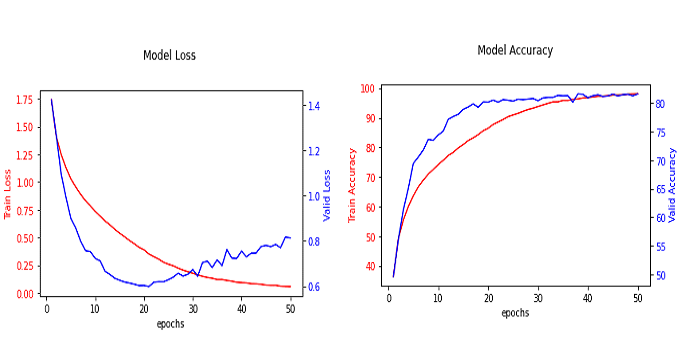
\includegraphics[width=0.9\linewidth]{./image_chapitre3/figure_14}
		\caption[Courbes de pr�cision et de perte du 2�me mod�le avec SGD, lr=0.001]{Courbes de pr�cision et de perte du 2�me mod�le avec \textbf{SGD}, $lr=0.001$}
		\label{fig:figure_3_14}
	\end{figure}
\end{itemize}
\subsubsection*{Discussion des r�sultats}
Les tests effectu�s sur le 2eme mod�le ont montr� que les meilleurs r�sultats sont obtenus en utilisant l'optimiseur SGD qui atteint 82\% avec un $ lr = 0 $. 001. N�anmoins, les pr�cisions diminuent en baissant les valeurs de learning rate (78\% avec $ lr = 0.001 $ et 73\% avec $ lr = 0.0001 $).\\[0.5\baselineskip]
Malgr� sa popularit�, les tests effectu�s avec Adam sur le 2eme mod�le n'ont pas �t� satisfaisants. Bien qu'ils atteignent une pr�cision de 76\% avec un $ lr = 0.0001 $, l'apprentissage avec Adam a men� vers un surapprentissage assez rapidement, ne d�passant pas les dix it�rations, ainsi qu'une valeur de pr�cision qui ne d�passe pas les 10\% avec diff�rentes valeurs de learning rate. c
En ce qui concerne l'optimiseur Adadelta, le mod�le a atteint des valeurs de pr�cisions entre 74\%,72\%,42\% en diminuant la valeur du learning rate respectivement de 0.01, 0.001, 0.0001.\\[0.5\baselineskip]
L'utilisation prometteuse du SGD pourrait �tre am�lior�e en augmentant le nombre de donn�es, ce qui implique plus de calculs et donc requiert plus de ressources.\\[0.5\baselineskip]
\begin{center}
	\begin{tabular}{|l|l|}
		\hline
		Optimiseur & Pr�cision Max \\
		\hline
		SGD & 82\%  \\
		\hline
		Adadelta & 74\%  \\
		\hline
		Adam & 76\%  \\
		\hline
	\end{tabular}
	\captionof{table}{Les r�sultats obtenus par les diff�rents optimiseurs utilis�s dans le deuxi�me mod�le}
	\label{tab_05}
\end{center}
\subsection{Conclusion}
D'apr�s les diff�rentes exp�rimentations et configurations test�es, le meilleur taux de pr�cision a �t� obtenu avec l'architecture du mod�le 2 \textbf{(Max-pooling and fully-connected dropout)}, avec application du dropout sur les couches de pooling et des couches enti�rement connect�es, en utilisant l'optimiseur SGD avec un $lr=0.001$ Dans l'ensemble, cette derni�re a globalement surpass� les performances obtenues avec le mod�le1.Ce r�sultat nous a permis d'utiliser le mod�le 2 \textbf{(Max-pooling and fully-connected dropout)} dans le MC Dropout Test.
\subsection{R�sultats du MC Dropout test}
\begin{figure}[H]
	\centering
	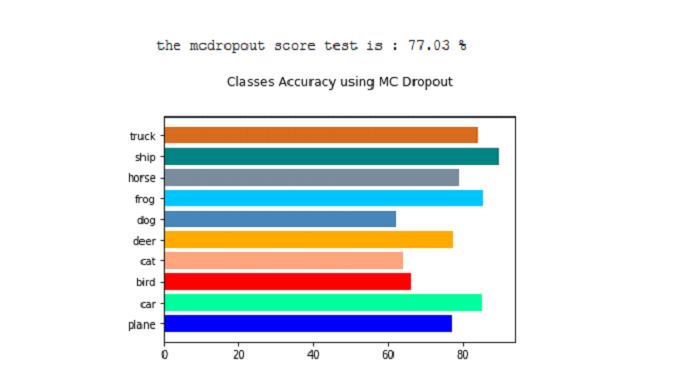
\includegraphics[width=0.9\linewidth]{./image_chapitre3/figure_15}
	\caption[Score du MC Dropout test et pr�cisions de chaque classe]{Score du MC Dropout test et pr�cisions de chaque classe}
	\label{fig:figure_3_15}
\end{figure}
On peut voir que le mod�le a atteint une pr�cision moyenne de 77\% sur les donn�es de test.\\[0.5\baselineskip]
On peut aussi visualiser les r�sultats de pr�cision de chaque classe qui varient entre un minimum de 63\% pour la classe � dog � et un maximum de 95\% pour la classe � ship �.
\newpage
\subsection{R�sultats d'incertitude du mod�le}
\begin{figure}[H]
	\centering
	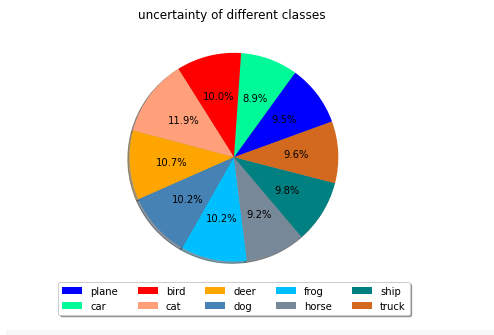
\includegraphics[width=0.9\linewidth]{./image_chapitre3/figure_16}
	\caption[Pourcentage d'incertitude des diff�rentes classes]{Pourcentage d'incertitude des diff�rentes classes}
	\label{fig:figure_3_16}
\end{figure}
On peut bien voir que l'incertitude de chaque classe ne d�passe pas les 11.9\%, et poss�de un taux minimal de 8.9\%.\\[0.5\baselineskip]
Ces r�sultats peuvent �tre tr�s utiles lors de la prise de d�cision car on peut am�liorer les r�sultats d'incertitude d'une classe donn�e en pr�voyant par exemple plus de donn�es en entr�e pour celle-ci pour permettre au mod�le de faire de bonnes pr�dictions, chose qui va nous permettre d'aboutir � un gain de temps �norme, �l�ment essentiel dans tout probl�me de prise de d�cision.\\[0.5\baselineskip]
\section{R�alisation de l'application}
En raison d'absence du mat�riel assez puissant, nous avons r�duit quelques param�tres de notre mod�le afin d'acc�l�rer le processus.\\[0.5\baselineskip]
Nous avons utilis� deux couches de convolution compos�es de 6 filtres chacun de taille 5x5, deux couches de max pooling de taille 2x2, trois couches enti�rement connect�es : La 1ere couche enti�rement connect�e utilise une fonction d'activation Relu et elle est compos�e de 120 neurones, la 2 �me utilise �galement une fonction d'activation Relu et est connect�e � la couche pr�c�dente avec 84 neurones et la 3 �me couche connect�es est li�e aux 84 sorties de la couche pr�c�dente pour pouvoir � la fin, g�n�rer 10 outputs.
\begin{figure}[H]
	\centering
	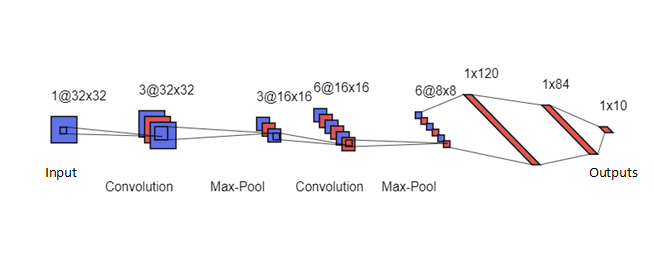
\includegraphics[width=0.9\linewidth]{./image_chapitre3/figure_17}
	\caption[Architecture du r�seau utilis� faite  � l'aide de l'outil : alexlenail.me]{Architecture du r�seau utilis� faite  � l'aide de l'outil : \textbf{alexlenail.me}}
	\label{fig:figure_3_17}
\end{figure}
Nous avons tenu � introduire notre r�seau de neurones profond bay�sien dans une interface graphique afin de pouvoir visualiser les performances facilement sans �tre oblig� de passer � chaque fois par les lignes de codes. Les d�tails de l'interface sont montr�s dans la figure suivante:
\begin{figure}[H]
	\centering
	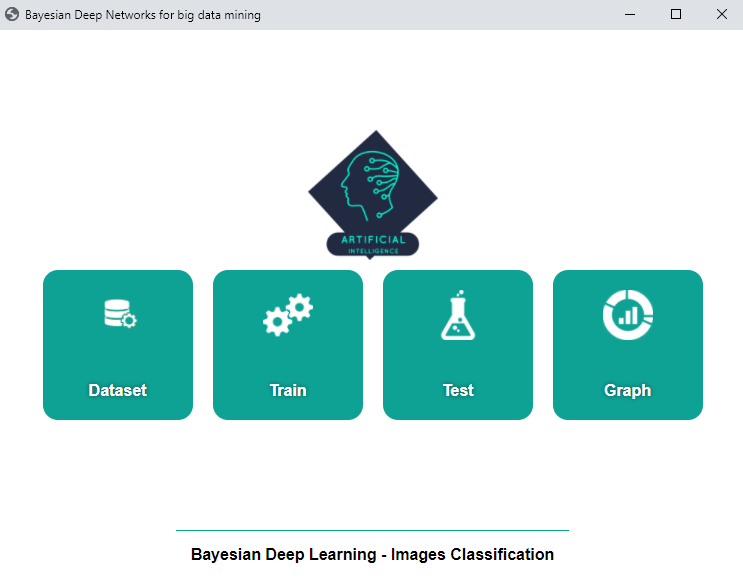
\includegraphics[width=0.9\linewidth]{./image_chapitre3/figure_18}
	\caption[L'interface de l'application]{L'interface de l'application}
	\label{fig:figure_3_18}
\end{figure}
\newpage
\begin{itemize}
	\item[\ding{228}] Dataset: un petit aper�u sur la data set utilis�e.
	Il est tr�s important de visualiser nos donn�es avant l'entrainement. Elles peuvent donner un aper�u des raisons pour lesquelles le mod�le ne se comporte pas comme pr�vu. Il peut y avoir des situations o� les donn�es du mod�le appartiennent enti�rement ou principalement � une classe, c'est-�-dire des situations o� le mod�le est biais�. Cela est principalement d� � un ensemble de donn�es d�s�quilibr�. Ainsi qu'au probl�me de manque de donn�es pour renforcer l'�nonc� du probl�me \cite{web26}.
\end{itemize}
\begin{figure}[H]
	\centering
	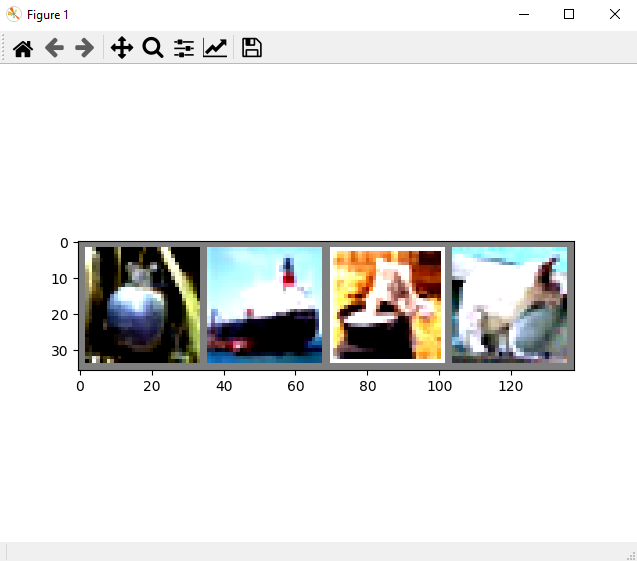
\includegraphics[width=0.9\linewidth]{./image_chapitre3/figure_19}
	\caption[Affichage d'un ensemble al�atoire des images d'entrainement]{Affichage d'un ensemble al�atoire des images d'entrainement}
	\label{fig:figure_3_19}
\end{figure}
\newpage
\begin{figure}[H]
	\centering
	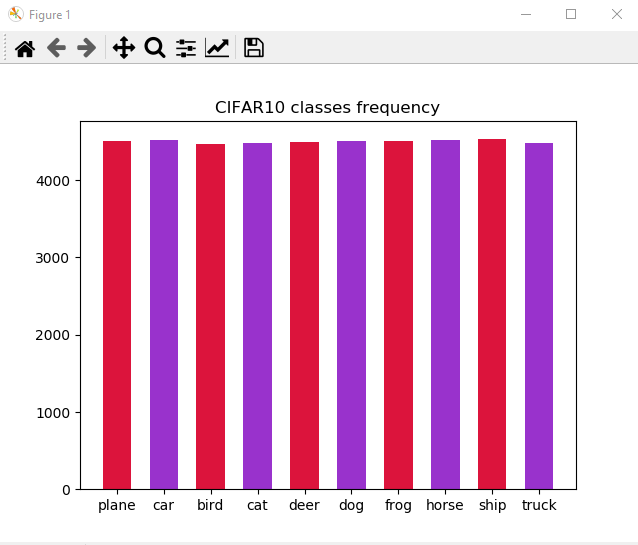
\includegraphics[width=0.9\linewidth]{./image_chapitre3/figure_20}
	\caption[distribution des images d'entrainement par classe]{distribution des images d'entrainement par classe}
	\label{fig:figure_3_20}
\end{figure}
\begin{itemize}
	\item[\ding{228}] train: lancement de l'apprentissage (affichage de la perte et de la pr�cision)
\end{itemize}
\begin{figure}[H]
	\centering
	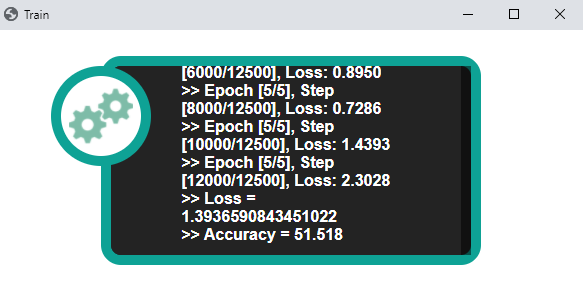
\includegraphics[width=0.9\linewidth]{./image_chapitre3/figure_21}
	\caption[La phase d'entrainement]{La phase d'entrainement}
	\label{fig:figure_3_21}
\end{figure}
\newpage
\begin{itemize}
	\item[\ding{228}] Graph : visualisation graphique de pr�cision et de perte pendant la phase d'entrainement.
\end{itemize}
\begin{figure}[H]
	\centering
	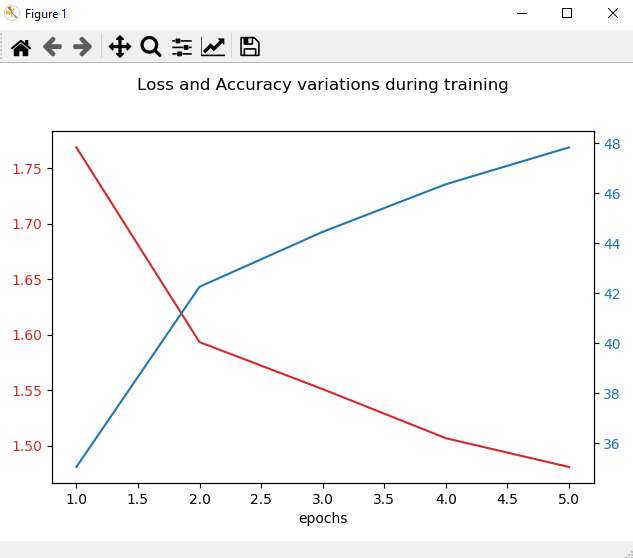
\includegraphics[width=0.9\linewidth]{./image_chapitre3/figure_22}
	\caption[La pr�cision et la perte durant la phase d'entrainement]{La pr�cision et la perte durant la phase d'entrainement}
	\label{fig:figure_3_22}
\end{figure}
\newpage
\begin{itemize}
	\item[\ding{228}] Test : lancement du test MC Dropout (affichage de la pr�cision et d'incertitude pour chaque classe).
\end{itemize}
\begin{figure}[H]
	\centering
	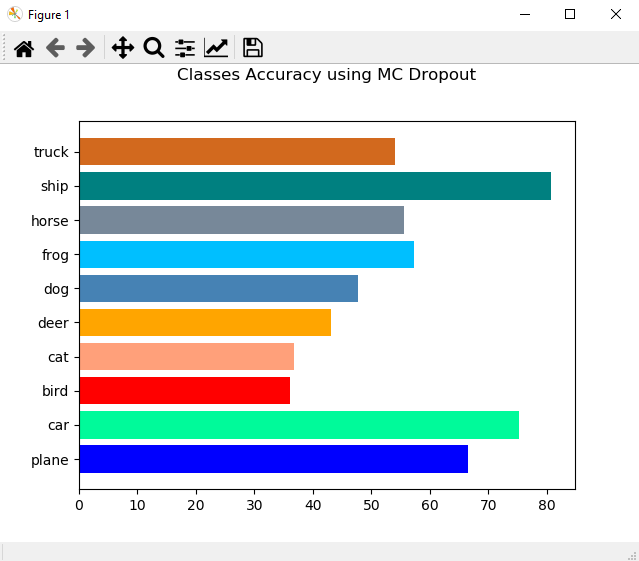
\includegraphics[width=0.7\linewidth]{./image_chapitre3/figure_23}
	\caption[La pr�cision de chaque classe durant la phase du test : Application]{La pr�cision de chaque classe durant la phase du test : Application}
	\label{fig:figure_3_23}
\end{figure}
\newpage
\begin{figure}[H]
	\centering
	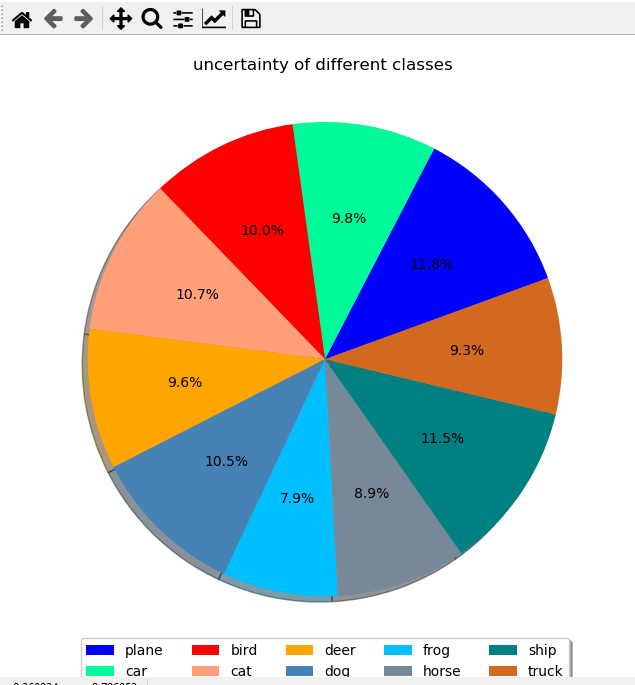
\includegraphics[width=0.7\linewidth]{./image_chapitre3/figure_24}
	\caption[Pourcentage d'incertitude de diff�rentes classes : Application]{Pourcentage d'incertitude de diff�rentes classes : Application}
	\label{fig:figure_3_24}
\end{figure}

\indent Le code source de l'application et du rapport de m�moire r�dig� en Latex sont disponibles dans le d�p�t distant (Github) suivant :\\
\url{https://github.com/merahsamia/PFE_BayesianDeepNetworksForBigDataMining}
\section{conclusion}
Dans ce chapitre nous avons pr�sent� les diff�rentes exp�rimentations ainsi que notre m�thodologie d'ex�cution et les diff�rentes architectures des mod�les utilis�s, avant de pr�senter les r�sultats obtenus. Enfin, nous avons montr� l'int�gration de ces r�sultats dans notre application � travers une interface utilisateur.






\include{pagevide}

%-----------------------Conclusion-----------------------%
\fancyhead[LE,RO]{} \fancyhead[LO]{}\fancyhead[RE]{}
\fancyhead[C]{\bfseries Conclusion g�n�rale}
\renewcommand{\footrulewidth}{0.5pt}
\phantomsection
\addcontentsline{toc}{chapter}{\numberline{}Conclusion g�n�rale}
\chapter*{Conclusion g�n�rale}
L'explosion quantitative des donn�es a oblig� les chercheurs � trouver de nouvelles mani�res robustes de voir et d'analyser le monde des donn�es, d'o� la prise en compte des r�seaux profonds bay�siens.\\[0.5\baselineskip]
\par Le r�seau profond bay�sien offre une nouvelle approche bas�e sur la notion d'incertitudes qui r�pond � la question : "Quelle est la fiabilit� de ma pr�diction ?". Cependant, dans leur forme classique, les r�seaux bay�siens �taient difficiles � impl�menter de par la complexit� spatiale et temporelle de la phase d'entra�nement (respectivement espace de stockage et temps d'ex�cution n�cessaire � un entra�nement). Les d�savantages techniques de ces m�thodes ont longtemps mis � l'�cart l'apprentissage profond bay�sien de la r�volution de l'intelligence artificielle dans laquelle nous vivons actuellement. Cependant, le MC Dropout remet � l'honneur ce pan de l'apprentissage automatique en s'adaptant directement � tout r�seau d�j� entra�n�. Il semble aujourd'hui possible d'attribuer un degr� de confiance � un r�seau de neurones.\\[0.5\baselineskip]
\par Dans le pr�sent m�moire, nous avons d'abord d�fini et pr�sent� ce que c'est l'apprentissage automatique et, de mani�re plus pr�cise, les r�seaux de neurones, avant d'exposer les diff�rentes techniques d'apprentissage et notions li�es au deep learning, ainsi que des g�n�ralit�s sur les r�seaux bay�siens. Et ce, afin d'enlever l'ambigu�t� quant � leurs diff�rents concepts pour cerner de mani�re pertinente les possibilit�s d'exploitation de leurs techniques.\\[0.5\baselineskip]
\par Nous avons ensuite effectu� un travail de recherche ardu sur l'�tat de l'art des r�seaux profonds bay�siens. Nous avons ainsi identifi� les travaux les plus fiables ainsi que les diff�rentes techniques et nouveaux concepts introduits et utilis�s au fil des avanc�es dans la recherche, afin d'y trouver les plus performants et int�ressants dans notre projet. Cependant, un des principaux freins au projet lors de cette phase a �t� le manque de ressources, l'int�r�t des chercheurs est assez r�cent, non pas seulement pour le big data d'ailleurs. Nous avons pass� beaucoup de temps � lire et � �tudier les publications et les articles pour voir ce qui se fait de mieux pour pouvoir concevoir notre propre mod�le.\\[0.5\baselineskip]
\par Nous avons �t� confront�s � quelques probl�mes dans la phase d'impl�mentation. Parmi ces probl�mes : l'absence de mat�riels assez cons�quents pour nous permettre d'explorer et d'exp�rimenter davantage les nombreux nouveaux concepts et techniques introduits ces derni�res ann�es et fa�onnant le d�veloppement de la recherche. L'utilisation d'un CPU a fait que le temps d'ex�cution �tait trop couteux. Afin de r�gler ce probl�me on doit utiliser des r�seaux de neurones plus profonds d�ploy�s sur un GPU au lieu d'un CPU sur des bases plus importantes.\\[0.5\baselineskip]
\par Pendant ce PFE, et avec la fermeture des �tablissements au niveau national afin de pr�venir la propagation du coronavirus, nous avons appris � travailler � distance avec l'�tablissement CERIST (Centre de recherche sur l'information scientifique et technique),  �a nous a �t�  b�n�fique, car cela nous a permis de gagner en flexibilit� du rythme et d'organisation et d'apprendre comment compter sur soi pour r�soudre les probl�mes au cas o� ils se pr�sentent et comment �tre m�ticuleux dans notre travail.\\[0.5\baselineskip]
\par Nous pouvons dire � pr�sent que notre objectif a �t� atteint, puisque l'application que nous avons r�alis�e satisfait les ambitions d�finies en premier lieu.\\[0.5\baselineskip]
\par Toutefois, il est important de noter qu'il ne s'agit que d'un premier aper�u de ce que pourrait r�ellement �tre un r�seau profond bay�sien et que la solution propos�e reste largement perfectible, on peut dire que ce travail n'est que dans sa version initiale mais �a nous a permis de mettre en pratique nos connaissances sur les r�seaux de neurones et les r�seaux bay�siens et d'en acqu�rir d'autres et le temps pass� � lire des articles nous a servi d'une bonne initiation � la recherche.





%----------------------Bibliographie---------------------%
\fancyhead[LE,RO]{} \fancyhead[LO]{}\fancyhead[RE]{}
\fancyhead[C]{\bfseries Bibliographie}
\renewcommand{\footrulewidth}{0.5pt}
\phantomsection
\renewcommand\bibname{Bibliographie}
\addcontentsline{toc}{chapter}{\numberline{}Bibliographie}
\begin{thebibliography}{9}
\expandafter\ifx\csname fonteauteurs\endcsname\relax
\def\fonteauteurs{\scshape}\fi

\bibitem[\bfseries Alexandre Perrot, novembre 2017]{ref01}
\newblock La visualisation d'information � l'�re du Big Data : r�soudre les probl�mes de scalabilit� par l'abstraction multi �chelle, th�se de doctorat L'UNIVERSIT� DE BORDEAUX.

\bibitem[\bfseries ALEXEI GRINBAUM, juin 2017]{ref02}
\newblock Clefs - \#64 - Les voix de la recherche VOYAGE AU COEUR DU BIG DATA, Big Data : de quoi parle-t-on ?

\bibitem[\bfseries Corentin HARDY, Avril 2019]{ref03}
\newblock Contribution au d�veloppement de l'apprentissage profond dans les syst�mes distribu�s, th�se de doctorat, L'UNIVERSITE DE RENNES 1 COMUE UNIVERSITE BRETAGNE LOIRE.


\bibitem[\bfseries Bernard ESPINASSE et Patrice BELLOT, 2017]{ref04} 
\newblock Introduction au Big Data Opportunit�s, stockage et analyse des m�gadonn�es, R�f. : H6040 V1.

\bibitem[\bfseries Mat, 2012]{ref05}
\newblock Mathieu, Gaetan, Benoit, St�phane. Fouille des r�seaux sociaux en ligne.Synth�se bibliographique sur le data mining sociale.2012.

\bibitem[\bfseries Ork, 2012]{ref06}
\newblock Orkhan Jafaro et Subhan Grismov. Machine Learning rapport de projet dans le cadre d'un master 2 informatique-universit� de Franche-Comt�, France 2012.

\bibitem[\bfseries R�mi Connesson, 2018]{ref07}
\newblock Le Deep Learning, comment fonctionne l'algorithme qui a bouscul� le monde de l'intelligence artificielle. Le blog de la School of AI en France.

\bibitem[\bfseries McCulloch, W.S. \& Pitts, 1943]{ref08}
\newblock McCulloch, W.S. \& Pitts, W. (1943). Bulletin of Mathematical Biophysics.

\bibitem[\bfseries Rosenblatt, 1958]{ref09}
\newblock Rosenblatt, F. (1958) The Perceptron: A Probabilistic Model for Information Storage and Organization in the Brain. Cornell Aeronautical Laboratory, Psychological Review, 65, 386-408.

\bibitem[\bfseries Chlo�-Agathe Azencott, 2019]{ref10}
\newblock Utilisez des mod�les supervis�s non lin�aires. OpenClassrooms.

\bibitem[\bfseries STEPHENE TUFFERY, 2019]{ref11}
\newblock Big Data, Machine Learning et apprentissage profond.

\bibitem[\bfseries Olivier Ezratty, Octobre 2017]{ref12}
\newblock Les usages de l'intelligence artificielle.

\bibitem[\bfseries Ian Goodfellow et al, 2016]{ref13}
\newblock Ian Goodfellow, Yoshua Bengio and Aaron Courville .Deep Learning. Convolutional Neural Networks, page 329.

\bibitem[\bfseries Andrej Karpathy, 2019]{ref14}
\newblock Stanford CS class CS231n: Convolutional Neural Networks for Visual Recognition.

\bibitem[\bfseries Radford et al, 2015]{ref15}
\newblock Radford, A., Metz, L., \& Chintala, S. (2015). Unsupervised representation learning with deep convolutional generative adversarial networks. arXiv preprint arXiv:1511.06434.

\bibitem[\bfseries Bengio et al., 2014]{ref16}
\newblock Bengio, Y., Laufer, E., Alain, G., \& Yosinski, J. (2014, January). Deep generative stochastic networks trainable by backprop. In International Conference on Machine Learning (pp. 226-234).

\bibitem[\bfseries Giorgio Roffo,2017]{ref17}
\newblock Ranking to Learn and Learning to Rank : On the Role of Ranking in Pattern Recognition Applications. Thesis for : European Doctor of Philosophy.

\bibitem[\bfseries Hasna Njah et al, 2016]{ref18}
\newblock Deep Bayesian network architecture for Big Data mining 

\bibitem[\bfseries David Bellot, 2002]{ref19}
\newblock Fusion de donn�es avec des r�seaux bay�siens pour la mod�lisation des syst�mes dynamiques et son application en t�l�m�decine Doctorat de l'universit� Henri Poincar� - Nancy 1

\bibitem[\bfseries Olivier Francois, 2006]{ref20}
\newblock De l'identification de structure de r�seaux bay�siens � la reconnaissance de formes � partir d'informations compl�tes ou incompl�tes.

\bibitem[\bfseries Pearl, 1985]{ref21}
\newblock J. Pearl et A. Paz. GRAPHOIDS : A graph-based logic for reasoning about relevance relations. Rapport technique (Cognitive Systems Laboratory, University of California, Los Angeles, 1985.

\bibitem[\bfseries Chong Wang et al, 2011]{ref22}
\newblock Chong Wang and David M. Blei. Collaborative topic modeling for recommending scientic articles. In KDD, pages 448?456, 2011.

\bibitem[\bfseries chr, 12]{ref23}
\newblock Christophe Thovex, R�seaux de comp�tences  de l'analyse des r�seaux sociaux � l'analyse pr�dictive de connaissances. Artificial intelligence, universit� de Nantes, France 2012

\bibitem[\bfseries Kostadin Georgiev et al, 2013]{ref24}
\newblock Kostadin Georgiev and Preslav Nakov. A non-iid framework for collaborative filtering with restricted Boltzmann machines. In ICML, pages 1148?1156, 2013.

\bibitem[\bfseries Na�m et al ,2007]{ref25}
\newblock Na�m, P., Wuillemin, P., Leray, P., Pourret, O., Becker, A., R�seaux bay�siens, 3e �d., Eyrolles, Paris, 2007, 424 p.

\bibitem[\bfseries Na�m et al ,2008]{ref26}
\newblock R�seaux bay�siens, Paris, Eyrolles

\bibitem[\bfseries Yiping Du, 2019]{ref27}
\newblock Bayesian Deep Convolutional Neural Network for SMS Quality Analysis.

\bibitem[\bfseries Pas,2009]{ref28}
\newblock Pascal Germain. Algorithmes d'apprentissage automatique inspir�s de la th�orie PAC-Bayes, Facult� des sciences et de G�nie, Universit� Laval, Qu�bec, Canada .2009

\bibitem[\bfseries Ruslan Salakhutdinove et al,  2007]{ref29}
\newblock Ruslan Salakhutdinove, Andriy Mnih, and Geoffrey E. Hinton. Restricted Boltzmann machines for collaborative ?ltering. In ICML, pages 791-798, 2007.

\bibitem[\bfseries Sachs et al, 2005]{ref30}
\newblock � Causal Protein-Signaling Networks Derived from Multiparameter Single-Cell Data �, Science, vol. 308, n� 5721, p. 523-529.

\bibitem[\bfseries Tristan St�rin ,2016]{ref31}
\newblock Tristan St�rin : R�seaux de neurones r�currents et m�moire : application � la musique.

\bibitem[\bfseries Kendall et Gal ,2017]{ref32}
\newblock Alex Kendall, Yarin Gal. What Uncertainties Do We Need in Bayesian Deep Learning for Computer Vision ?

\bibitem[\bfseries Raanan Y. Rohekar et al, 2018]{ref33}
\newblock Raanan Y. Rohekar, Shami Nisimov, Yaniv Gurwicz, Guy Koren Gal Novik, 2018 : Constructing Deep Neural Networks by Bayesian Network Structure Learning.

\bibitem[\bfseries Umara Zafar et al, 2019]{ref34}
\newblock Umara Zafar, Mubeen Ghafoor, Tehseen Zia, Ghufran Ahmed, Ahsan Latif, Kaleem Razzaq Malik and Abdullahi Mohamud Sharif. Face recognition with Bayesian convolutional networks for robust surveillance systems. EURASIP Journal on Image and Video Processing, EURASIP Journal on Image and Video Processing.

\bibitem[\bfseries Gal et Ghahramani, 2015]{ref35}
\newblock Yarin Gal, Zoubin Ghahramani. Bayesian Convolutional Neural Networks with Bernoulli Approximate Variational Inference.

\bibitem[\bfseries Alex Kendall et al., 2017]{ref36}
\newblock Alex Kendall, Vijay Badrinarayanan, Roberto Cipolla. Bayesian SegNet: Model Uncertainty in Deep Convolutional Encoder-Decoder Architectures for Scene Understanding.

\bibitem[\bfseries Gal et Ghahramani, 2016]{ref37}
\newblock Yarin Gal, Zoubin Ghahramani. Dropout as a Bayesian Approximation: Representing Model Uncertainty in Deep Learning.

\bibitem[\bfseries XIAO SUN et al, 2019]{ref38}
\newblock Xiao Sun, Jia Li, Xing Wei, Changliang Li, and Jianhua Tao. 2019. Emotional Conversation Generation Based on a Bayesian Deep Neural Network. ACM Trans. Inf. Syst. 38, 1, Article 8 (December 2019)

\bibitem[\bfseries Gal et al, 2017]{ref39}
\newblock Yarin Gal, Riashat Islam, Zoubin Ghahramani. Deep Bayesian Active Learning with Image Data.

\bibitem[\bfseries Shen et al, 2018]{ref40}
\newblock Yanyao Shen, Hyokun Yun, Zachary Chase Lipton, Yakov Kronrod. Deep Active Learning for Named Entity Recognition.

\bibitem[\bfseries Blundell et al, 2015]{ref41}
\newblock Charles Blundell, Julien Cornebise, Koray Kavukcuoglu, Daan Wierstra. Weight Uncertainty in Neural Networks.

\bibitem[\bfseries Deshpande, 2016]{ref42}
\newblock DESHPANDE, Adit, 2016. A Beginner?s Guide To Understanding Convolutional Neural Networks Part 2. In : [en ligne]. 17 2016. [Consult� le 21 aout 2020]. Disponible � l?adresse : \url{https://adeshpande3.github.io/A-Beginner%27s-Guide-To-UnderstandingConvolutional-Neural-Networks-Part-2/}.

\bibitem[\bfseries Srivastava et al, 2014]{ref43}
\newblock Nitish Srivastava, Geoffrey Hinton, Alex Krizhevsky, Ilya Sutskever, Ruslan Salakhutdinov, Dropout. A Simple Way to Prevent Neural Networks from Overfitting.

\bibitem[\bfseries Der Kiureghian et Ditlevsen, 2009]{ref44}
\newblock Aleatory or epistemic? does it matter? Structural Safety, 31(2):105?112.

\bibitem[\bfseries Ronald Seoh, 2020]{ref45}
\newblock Qualitative Analysis of Monte Carlo Dropout, University of Massachusetts Amherst.

\bibitem[\bfseries Gal, 2016]{ref46}
\newblock Yarin Gal. Uncertainty in deep learning. PhD thesis, PhD thesis, University of Cambridge, 2016.

\end{thebibliography}

%----------------------Webographie---------------------%
\fancyhead[LE,RO]{} \fancyhead[LO]{}\fancyhead[RE]{}
\fancyhead[C]{\bfseries Webographie}
\renewcommand{\footrulewidth}{0.5pt}
\phantomsection
\renewcommand\bibname{Webographie}
\addcontentsline{toc}{chapter}{\numberline{}Webographie}
\begin{thebibliography}{site5}

\bibitem[1]{web01}
LE DEEP LEARNING PAS � PAS : LES CONCEPTS (1/2). 
\newblock
\url{https://www.technologies-ebusiness.com/enjeux-et-tendances/le-deep-learning-pas-a-pas}.
\newblock [Consult{\'e}: 06/08/2020].

\bibitem[2]{web02}
Harry Pommier, 2020. [Fiche m�mo] R�seau de neurones profond.
\newblock
\url{https://medium.zenika.com/fiche-m%C3%A9mo-r%C3%A9seau-de-neurones-profond-66f6bf48a472}.
\newblock [Consult{\'e}: 25/08/2020].

\bibitem[3]{web03}
Mod�les bas�s sur le r�flex : apprentissage automatique
\newblock
\url{https://stanford.edu/~shervine/l/fr/teaching/cs-221/pense-bete-modeles-reflex}.
\newblock [Consult{\'e}: 08/08/2020].

\bibitem[4]{web04}
La r�tropropagation du gradient. 
\newblock
\url{https://dataanalyticspost.com/Lexique/retropropagation/#:~:text=La%20r%C3%A9tropropagation%20du%20gradient%20de,dans%20une%20base%20d'apprentissage}.
\newblock [Consult{\'e}: 12/08/2020].

\bibitem[5]{web05}
Thierry Maubant. Qu'est-ce que le surapprentissage ?
\newblock
\url{https://www.actuia.com/faq/quest-ce-que-le-surapprentissage/}.
\newblock [Consult{\'e}: 07/08/2020].

\bibitem[6]{web06}
Artificial intelligence and the rise of economec inequality
\newblock
\url{https://www.datascience.us/artificial-intelligence-rise-economic-inequality/}.
\newblock [Consult{\'e}: 15/08/2020].

\bibitem[7]{web07}
Afshine Amidi et Shervine Amidi. (2018). Pense-b�te de r�seaux de neurones convolutionnels.
\newblock
\url{https://stanford.edu/~shervine/l/fr/teaching/cs-230/pense-bete-reseaux-neurones-convolutionnels}.

\bibitem[8]{web08}
Convolutional Neural Networks (CNN): Step 3 -Flattening.
\newblock
\url{https://www.superdatascience.com/blogs/convolutional-neural-networks-cnn-step-3-flattening}.
\newblock [Consult{\'e}: 22/08/2020].

\bibitem[9]{web09}
Par Jean-Pierre Mistral.(2018)   BIG DATA, INTELLIGENCE ARTIFICIELLE, APPRENTISSAGE AUTOMATIQUE ET LE RGPD.
\newblock
\url{https://www.village-justice.com/articles/big-data-intelligence-artificielle-apprentissage-automatique-rgpd,26838.html}.
\newblock [Consult{\'e}: 19/08/2020].

\bibitem[10]{web10}
Yarin Gal. What My Deep Model Doesn't Know
\newblock
\url{http://mlg.eng.cam.ac.uk/yarin/blog_3d801aa532c1ce.html}.
\newblock [Consult{\'e}: 28/08/2020].

\bibitem[11]{web11}
Robin Camarasa. Bayesian Deep Learning : Soyez s�r de vos incertitudes.
\newblock
\url{https://www.datagenius.fr/post/bayesian-deep-learning-soyez-sur-de-vos-incertitudes}.
\newblock [Consult{\'e}: 26/08/2020].

\bibitem[12]{web12}
G�bor Vecsei. Experiments with Monte-Carlo dropout for uncertainty estimation.
\newblock
\url{https://www.gaborvecsei.com/Monte-Carlo-Dropout/}.
\newblock [Consult{\'e}: 26/08/2020].

\bibitem[13]{web13}
Deep learning Dropout technical analysis.
\newblock
\url{https://www.programmersought.com/article/31754654312/}.
\newblock [Consult{\'e}: 28/08/2020].

\bibitem[14]{web14}
Python.
\newblock
\url{https://fr.wikibooks.org/wiki/Programmation_Python/Introduction}.
\newblock [Consult{\'e}: 06/08/2020].

\bibitem[15]{web15}
Anaconda.
\newblock
\url{https://www.anaconda.com/what-is-anaconda/}.
\newblock [Consult{\'e}: 06/08/2020].

\bibitem[16]{web16}
Pytorch.
\newblock
\url{https://datafranca.org/wiki/PyTorch}.
\newblock [Consult{\'e}: 06/08/2020].

\bibitem[17]{web17}
Numpy.
\newblock
\url{https://openclassrooms.com/fr/courses/4452741-decouvrez-les-librairies-python-pour-la-data-science/4740941-plongez-en-detail-dans-la-librairie-numpy}.
\newblock [Consult{\'e}: 06/08/2020].

\bibitem[18]{web18}
Matplotlib
\newblock
\url{https://matplotlib.org/}.
\newblock [Consult{\'e}: 06/08/2020].

\bibitem[19]{web19}
HTML Tutorial.
\newblock
\url{https://www.w3schools.com/html/}.
\newblock [Consult{\'e}: 04/09/2020].

\bibitem[20]{web20}
CSS Tutorial.
\newblock
\url{https://www.w3schools.com/css/}.
\newblock [Consult{\'e}: 04/09/2020].

\bibitem[21]{web21}
JavaScript Tutorial
\newblock
\url{https://www.w3schools.com/js/}.
\newblock [Consult{\'e}: 04/09/2020].

\bibitem[22]{web22}
Create HTML User Interface for Python using Eel Library
\newblock
\url{https://medium.com/wronmbertech/create-html-user-interface-for-python-using-eel-library-bab101cc0f99}.
\newblock [Consult{\'e}: 04/09/2020].

\bibitem[23]{web23}
Pycharm
\newblock
\url{https://www.jetbrains.com/fr-fr/pycharm/}.
\newblock [Consult{\'e}: 06/08/2020].

\bibitem[24]{web24}
Jupyter.
\newblock
\url{https://jupyter-notebook.readthedocs.io/en/stable/}.
\newblock [Consult{\'e}: 06/08/2020].

\bibitem[25]{web25}
Cifar 10
\newblock
\url{http://www.cs.toronto.edu/~kriz/cifar.html}.
\newblock [Consult{\'e}: 06/08/2020].

\bibitem[26]{web26}
Useful Plots to Diagnose your Neural Network.
\newblock
\url{https://towardsdatascience.com/useful-plots-to-diagnose-your-neural-network-521907fa2f45}.
\newblock [Consult{\'e}: 28/08/2020].

\end{thebibliography}

%----------------------Webographie---------------------%
%\fancyhead[LE,RO]{} \fancyhead[LO]{}\fancyhead[RE]{}
%\fancyhead[C]{\bfseries Bibliographie - Webographie}
%\renewcommand{\footrulewidth}{0.5pt}
%\phantomsection
%\renewcommand\bibname{Webographie}
%\addcontentsline{toc}{chapter}{\numberline{} Webographie}
%\begin{thebibliography}{site5}

\bibitem[1]{web01}
LE DEEP LEARNING PAS � PAS : LES CONCEPTS (1/2). 
\newblock
\url{https://www.technologies-ebusiness.com/enjeux-et-tendances/le-deep-learning-pas-a-pas}.
\newblock [Consult{\'e}: 06/08/2020].

\bibitem[2]{web02}
Harry Pommier, 2020. [Fiche m�mo] R�seau de neurones profond.
\newblock
\url{https://medium.zenika.com/fiche-m%C3%A9mo-r%C3%A9seau-de-neurones-profond-66f6bf48a472}.
\newblock [Consult{\'e}: 25/08/2020].

\bibitem[3]{web03}
Mod�les bas�s sur le r�flex : apprentissage automatique
\newblock
\url{https://stanford.edu/~shervine/l/fr/teaching/cs-221/pense-bete-modeles-reflex}.
\newblock [Consult{\'e}: 08/08/2020].

\bibitem[4]{web04}
La r�tropropagation du gradient. 
\newblock
\url{https://dataanalyticspost.com/Lexique/retropropagation/#:~:text=La%20r%C3%A9tropropagation%20du%20gradient%20de,dans%20une%20base%20d'apprentissage}.
\newblock [Consult{\'e}: 12/08/2020].

\bibitem[5]{web05}
Thierry Maubant. Qu'est-ce que le surapprentissage ?
\newblock
\url{https://www.actuia.com/faq/quest-ce-que-le-surapprentissage/}.
\newblock [Consult{\'e}: 07/08/2020].

\bibitem[6]{web06}
Artificial intelligence and the rise of economec inequality
\newblock
\url{https://www.datascience.us/artificial-intelligence-rise-economic-inequality/}.
\newblock [Consult{\'e}: 15/08/2020].

\bibitem[7]{web07}
Afshine Amidi et Shervine Amidi. (2018). Pense-b�te de r�seaux de neurones convolutionnels.
\newblock
\url{https://stanford.edu/~shervine/l/fr/teaching/cs-230/pense-bete-reseaux-neurones-convolutionnels}.

\bibitem[8]{web08}
Convolutional Neural Networks (CNN): Step 3 -Flattening.
\newblock
\url{https://www.superdatascience.com/blogs/convolutional-neural-networks-cnn-step-3-flattening}.
\newblock [Consult{\'e}: 22/08/2020].

\bibitem[9]{web09}
Par Jean-Pierre Mistral.(2018)   BIG DATA, INTELLIGENCE ARTIFICIELLE, APPRENTISSAGE AUTOMATIQUE ET LE RGPD.
\newblock
\url{https://www.village-justice.com/articles/big-data-intelligence-artificielle-apprentissage-automatique-rgpd,26838.html}.
\newblock [Consult{\'e}: 19/08/2020].

\bibitem[10]{web10}
Yarin Gal. What My Deep Model Doesn't Know
\newblock
\url{http://mlg.eng.cam.ac.uk/yarin/blog_3d801aa532c1ce.html}.
\newblock [Consult{\'e}: 28/08/2020].

\bibitem[11]{web11}
Robin Camarasa. Bayesian Deep Learning : Soyez s�r de vos incertitudes.
\newblock
\url{https://www.datagenius.fr/post/bayesian-deep-learning-soyez-sur-de-vos-incertitudes}.
\newblock [Consult{\'e}: 26/08/2020].

\bibitem[12]{web12}
G�bor Vecsei. Experiments with Monte-Carlo dropout for uncertainty estimation.
\newblock
\url{https://www.gaborvecsei.com/Monte-Carlo-Dropout/}.
\newblock [Consult{\'e}: 26/08/2020].

\bibitem[13]{web13}
Deep learning Dropout technical analysis.
\newblock
\url{https://www.programmersought.com/article/31754654312/}.
\newblock [Consult{\'e}: 28/08/2020].

\bibitem[14]{web14}
Python.
\newblock
\url{https://fr.wikibooks.org/wiki/Programmation_Python/Introduction}.
\newblock [Consult{\'e}: 06/08/2020].

\bibitem[15]{web15}
Anaconda.
\newblock
\url{https://www.anaconda.com/what-is-anaconda/}.
\newblock [Consult{\'e}: 06/08/2020].

\bibitem[16]{web16}
Pytorch.
\newblock
\url{https://datafranca.org/wiki/PyTorch}.
\newblock [Consult{\'e}: 06/08/2020].

\bibitem[17]{web17}
Numpy.
\newblock
\url{https://openclassrooms.com/fr/courses/4452741-decouvrez-les-librairies-python-pour-la-data-science/4740941-plongez-en-detail-dans-la-librairie-numpy}.
\newblock [Consult{\'e}: 06/08/2020].

\bibitem[18]{web18}
Matplotlib
\newblock
\url{https://matplotlib.org/}.
\newblock [Consult{\'e}: 06/08/2020].

\bibitem[19]{web19}
HTML Tutorial.
\newblock
\url{https://www.w3schools.com/html/}.
\newblock [Consult{\'e}: 04/09/2020].

\bibitem[20]{web20}
CSS Tutorial.
\newblock
\url{https://www.w3schools.com/css/}.
\newblock [Consult{\'e}: 04/09/2020].

\bibitem[21]{web21}
JavaScript Tutorial
\newblock
\url{https://www.w3schools.com/js/}.
\newblock [Consult{\'e}: 04/09/2020].

\bibitem[22]{web22}
Create HTML User Interface for Python using Eel Library
\newblock
\url{https://medium.com/wronmbertech/create-html-user-interface-for-python-using-eel-library-bab101cc0f99}.
\newblock [Consult{\'e}: 04/09/2020].

\bibitem[23]{web23}
Pycharm
\newblock
\url{https://www.jetbrains.com/fr-fr/pycharm/}.
\newblock [Consult{\'e}: 06/08/2020].

\bibitem[24]{web24}
Jupyter.
\newblock
\url{https://jupyter-notebook.readthedocs.io/en/stable/}.
\newblock [Consult{\'e}: 06/08/2020].

\bibitem[25]{web25}
Cifar 10
\newblock
\url{http://www.cs.toronto.edu/~kriz/cifar.html}.
\newblock [Consult{\'e}: 06/08/2020].

\bibitem[26]{web26}
Useful Plots to Diagnose your Neural Network.
\newblock
\url{https://towardsdatascience.com/useful-plots-to-diagnose-your-neural-network-521907fa2f45}.
\newblock [Consult{\'e}: 28/08/2020].

\end{thebibliography}
%--------------------------Page vide---------------------%
\include{pagevide}\fancyhf{}
\renewcommand{\headrulewidth}{0pt}%
\renewcommand{\footrulewidth}{0pt}

\end{document}
